\chapter[Curvature Measures]{Curvature Measures of Nonlinearity}

\prologue{``The great tragedy of Science:  the slaying of a beautiful
hypothesis by an ugly fact.''}{Thomas Huxley}


In Chapter 2 we presented linear approximation
inference intervals and  regions for parameters in
nonlinear regression models,
and in Chapter 6 we discussed improved
methods for summarizing inferences about the parameters.
An important assumption used in the development of these methods
is that the expectation surface is flat (the planar assumption),
so that the tangent plane provides an accurate approximation.
In this chapter, we develop relative curvature measures of the
\index{curvature!measures of nonlinearity}
\index{nonlinearity!relative curvature measures}
nonlinearity of an estimation
situation, and discuss how they can be used to indicate the
adequacy of the linear approximation in a particular case.
We then apply the curvature measures to 67 real data set--model
combinations to gain some idea of how serious the two kinds of
nonlinearity are in practice.
Finally, we discuss more direct assessment of intrinsic nonlinearity
to provide practical justification for assuming planarity.

As discussed in Section 2.5, linear approximation inference
regions can be obtained from a first order Taylor
series approximation to the expectation function evaluated at
\index{linear approximation!to expectation function}
\index{expectation function!linear approximation to}
$\hat \btheta$.
The $1 - \alpha$ region is
\begin{equation}
  ( \btheta - \hat \btheta ) \trans \hat \bV \trans \hat \bV ( \btheta
  - \hat \btheta ) \le P s^2 \FPNP
  \label{eqn:linreg}
\end{equation}
where $\hat \bV$ is the derivative matrix evaluated at $\hat \btheta$.

Geometrically, the linear approximation inference region (\#eqn linreg\#)
\index{linear approximation!inference region}
\index{linear approximation!to expectation surface}
\index{expectation surface!linear approximation to}
\index{expectation surface!tangent plane}
\index{tangent plane!approximation to expectation surface}
assumes that, over the region of interest, the mapping of
$\btheta$ to $\boeta ( \btheta )$ is
$$
\hat{\boeta}+ \hat{\bV}( \btheta - \hat{\btheta})
$$
This approximation, as pointed out by
\citeasnoun{beal:1960} and as
%\glossary{ Beale, E.M.L.}
discussed in Section 2.5, will be good only if the expectation
\index{planar!assumption}
\index{assumptions!planar}
surface is sufficiently flat to be replaced by the tangent plane,
and if straight, parallel equispaced lines in the parameter space
\index{assumptions!uniform coordinate}
\index{uniform coordinate!assumption}
map into nearly straight, parallel equispaced lines on the
expectation surface.
In that event, we can assume that the expectation surface
inference region is a sphere of radius
$\sqrt {P s^2 \FPNP}$
on the tangent plane and that the mapping of the
tangent plane to the parameter space is linear.

To determine how planar the expectation surface is, and how
uniform the parameter lines are on the tangent plane, we use
second derivatives of the expectation function to derive
{\em curvature measures\/} of {\em intrinsic\/} and
{\em parameter effects nonlinearity}.
The curvatures can also be used to investigate
reparametrizations of expectation functions so as to obtain
models which have more valid linear approximation parameter
inference regions.

\section{Velocity and Acceleration Vectors}

A fundamental feature of linear models is that second and higher
order derivatives of the expectation function with respect to the
parameters are zero.
It is logical, therefore, to attempt to measure the nonlinearity of a
model by investigating second order derivatives of the
expectation function \cite{beal:1960,bate:1978,bate:watt:1980}.
%\glossary{ Beale, E.M.L.}
%\glossary{ Bates, D.M.}
%\glossary{ Watts, D.G.}
For clarity, we introduce a dot notation to distinguish
between first and second derivatives.
Thus for a nonlinear model $\boeta ( \btheta )$, the $N \times P$
derivative matrix is written as $\dot{\bV}$ with elements
\index{derivative matrix}
\begin{equation}
  \lb \dot \bV \rb_{np} = {\partial f ( \bx_n , \btheta ) \over
  \partial \theta_p}
  \label{eqn:8.1}
\end{equation}
and the $N \times P \times P$ second derivative array is written as
$\ddot{\bV}$ with elements
\begin{equation}
  \lb \ddot{\bV}\rb_{npq} = {\partial^2 f ( \bx_n , \btheta ) \over
  \partial \theta_{p}\partial \theta_q}
  \label{eqn:8.2}
\end{equation}
In (\ref{eqn:8.1}) and (\ref{eqn:8.2}), $n$ runs from 1 to $N$
while $p$ and $q$ run from 1 to $P$.
In matrix notation,
$$
\dot{\bV} = {\partial \boeta  \over \partial \btheta \trans}
$$
where each row of $\dot{\bV}$ is the gradient of one coordinate of
$\boeta ( \btheta )$ with respect to $\btheta$.
Alternatively, we may regard $\dot{\bV}$ as consisting of
vectors $\dot{\bv}_p , p = 1, 2 ,\ldots, P$.

Also,
$$
\ddot{\bV}= {\partial^2 \boeta  \over \partial \btheta  \partial
\btheta \trans}
$$
where each face $\ddot{\bV}_n $ of $\ddot{\bV}$ is a complete
$P \times P$ second derivative matrix, or Hessian, of one element
\index{second derivative!array}
\index{array!second derivative}
\index{array!Hessian}
\index{Hessian!array}
of $\boeta ( \btheta )$ with respect to $\btheta$.
As above, we may regard the Hessian array as consisting
of vectors $\ddot{\bv}_{pq} , p,q= 1, 2 ,\ldots, P$.

The vectors $\dot{\bv}$ are, of course, the tangent vectors, and they
\index{vector!tangent}
are also called {\em velocity\/} vectors, since they give
the rate of change of $\boeta$ with respect to each parameter.
Accordingly, the vectors $\ddot{\bv}$ are called
{\em acceleration\/} vectors, since they give the rates of change
\index{acceleration!vector}
\index{vector!acceleration}
of the velocity vectors with respect to the parameters.
That is,
$$
\ddot{\bv}_{pq} = {\partial \dot{\bv}_p  \over \partial \theta_q}
$$

\begin{example}\label{mic:11}

For the Michaelis--Menten expectation function
$$
f ( x , \btheta ) = {\theta_1 x  \over  \theta_2 + x }
$$
the elements in $\dot{\bV}$ are
\begin{eqnarray*}
  \lb \dot{\bV} \rb_{n1}&=&{x_n \over \theta_2 + x_n }\\
  \lb \dot{\bV}\rb_{n2}&=&{ - \theta_1 x_n \over (\theta_2 + x_n)^2 }
\end{eqnarray*}
Evaluating these functions at each $x_{n}$ value for a
particular parameter pair $\btheta$ produces the matrix $\dot{\bV}$.

The elements in $\ddot{\bV}$ can also be evaluated, as
\begin{eqnarray*}
  \lb \ddot{\bV}\rb_{n11}&=&0  \\
  \lb \ddot{\bV}\rb_{n12}&=&{-x_n\over(\theta_2+x_n)^2 }\\
  \lb \ddot{\bV}\rb_{n21}&=&\lb\ddot{\bV}\rb_{n12}\\
  \lb \ddot{\bV}\rb_{n22}&=&{2\theta_1 x_n\over(\theta_2+x_n)^3}
\end{eqnarray*}

For the Puromycin data, the concentrations and the velocity and
acceleration
vectors at $\hat \btheta$'-1p' are given in Table~\ref{tbl:PURaccel}.
\begin{table}
  \caption{\label{tbl:PURaccel}
  Velocity and acceleration vectors for the Puromycin data evaluated
  at $\hat{\btheta}=(212.7,0.0641) \trans$.}
  \begin{center}
    \begin{tabular}{r r r r r}
      \mbox{}
\par\vspace{0.5\baselineskip}
%c  c s c s s
%c  c s c s s
%c  c c c c c
%n  n n n n n.
%\_
%:Velocity:Acceleration
%::
%Conc.:$\dot \bv_\dot {1}$:$\bv_\ddot {2}$:$\bv_\ddot {11}$:$\bv_\ddot {12}$:$\bv}_{22$
%\par\vspace{4.0pt}
%\_
%0.02:0.237812:--601.458:0:--2.82773:14303.4
%0.02:0.237812:--601.458:0:--2.82773:14303.4
%0.06:0.483481:--828.658:0:--3.89590:13354.7
%0.06:0.483481:--828.658:0:--3.89590:13354.7
%0.11:0.631821:--771.903:0:--3.62907:8867.4
%0.11:0.631821:--771.903:0:--3.62907:8867.4
%0.22:0.774375:--579.759:0:--2.72571:4081.4
%0.22:0.774375:--579.759:0:--2.72571:4081.4
%0.56:0.897292:--305.807:0:--1.43774:980.0
%0.56:0.897292:--305.807:0:--1.43774:980.0
%1.10:0.944936:--172.655:0:--\/0.81173:296.6
%1.10:0.944936:--172.655:0:--\/0.81173:296.6
%\par\vspace{2.0pt}
%\_
    \end{tabular}
  \end{center}
\end{table}
\end{example}

\subsection{Tangential and Normal Accelerations}
\index{acceleration!tangential}
\index{acceleration!normal}

The acceleration vectors can be decomposed into components
{\em in\/} and {\em orthogonal to\/} the tangent plane.
Because there are only $P ( P + 1 ) / 2$ distinct acceleration
vectors, the acceleration vectors will span a subspace of maximum
dimension $P ( P + 1 ) / 2$ in the response space, so the
maximum dimension of the combined tangent and acceleration spaces
is $P ( P + 3 ) / 2$
\index{tangent!space dimension}
\index{acceleration!space dimension}
\cite{hami:1980}.
%\glossary{ Hamilton, D.C.}
In many cases the combined dimension is only slightly larger than $P$,
say $P + P'$.

\begin{example}\label{mic:12}

For the Michaelis--Menten model,
$\ddot{\bv}_{11} \equiv  {\bf 0} $ because $\theta_{1}$ is a
conditionally linear parameter.
This conditional linearity causes the
acceleration vector $\ddot{\bv}_{12} = \ddot{\bv}_{21}$ to be
a simple multiple of $\dot{\bv}_{2}$, so that the only acceleration
vector which is not in the tangent plane is $\ddot{\bv}_{22}$.
The tangent space has dimension 2, the acceleration space has
dimension 2, and the combined tangent and acceleration spaces
have dimension 3.

In Figure \ref{fig:PURtanvec}
\begin{figure}
  \centerline{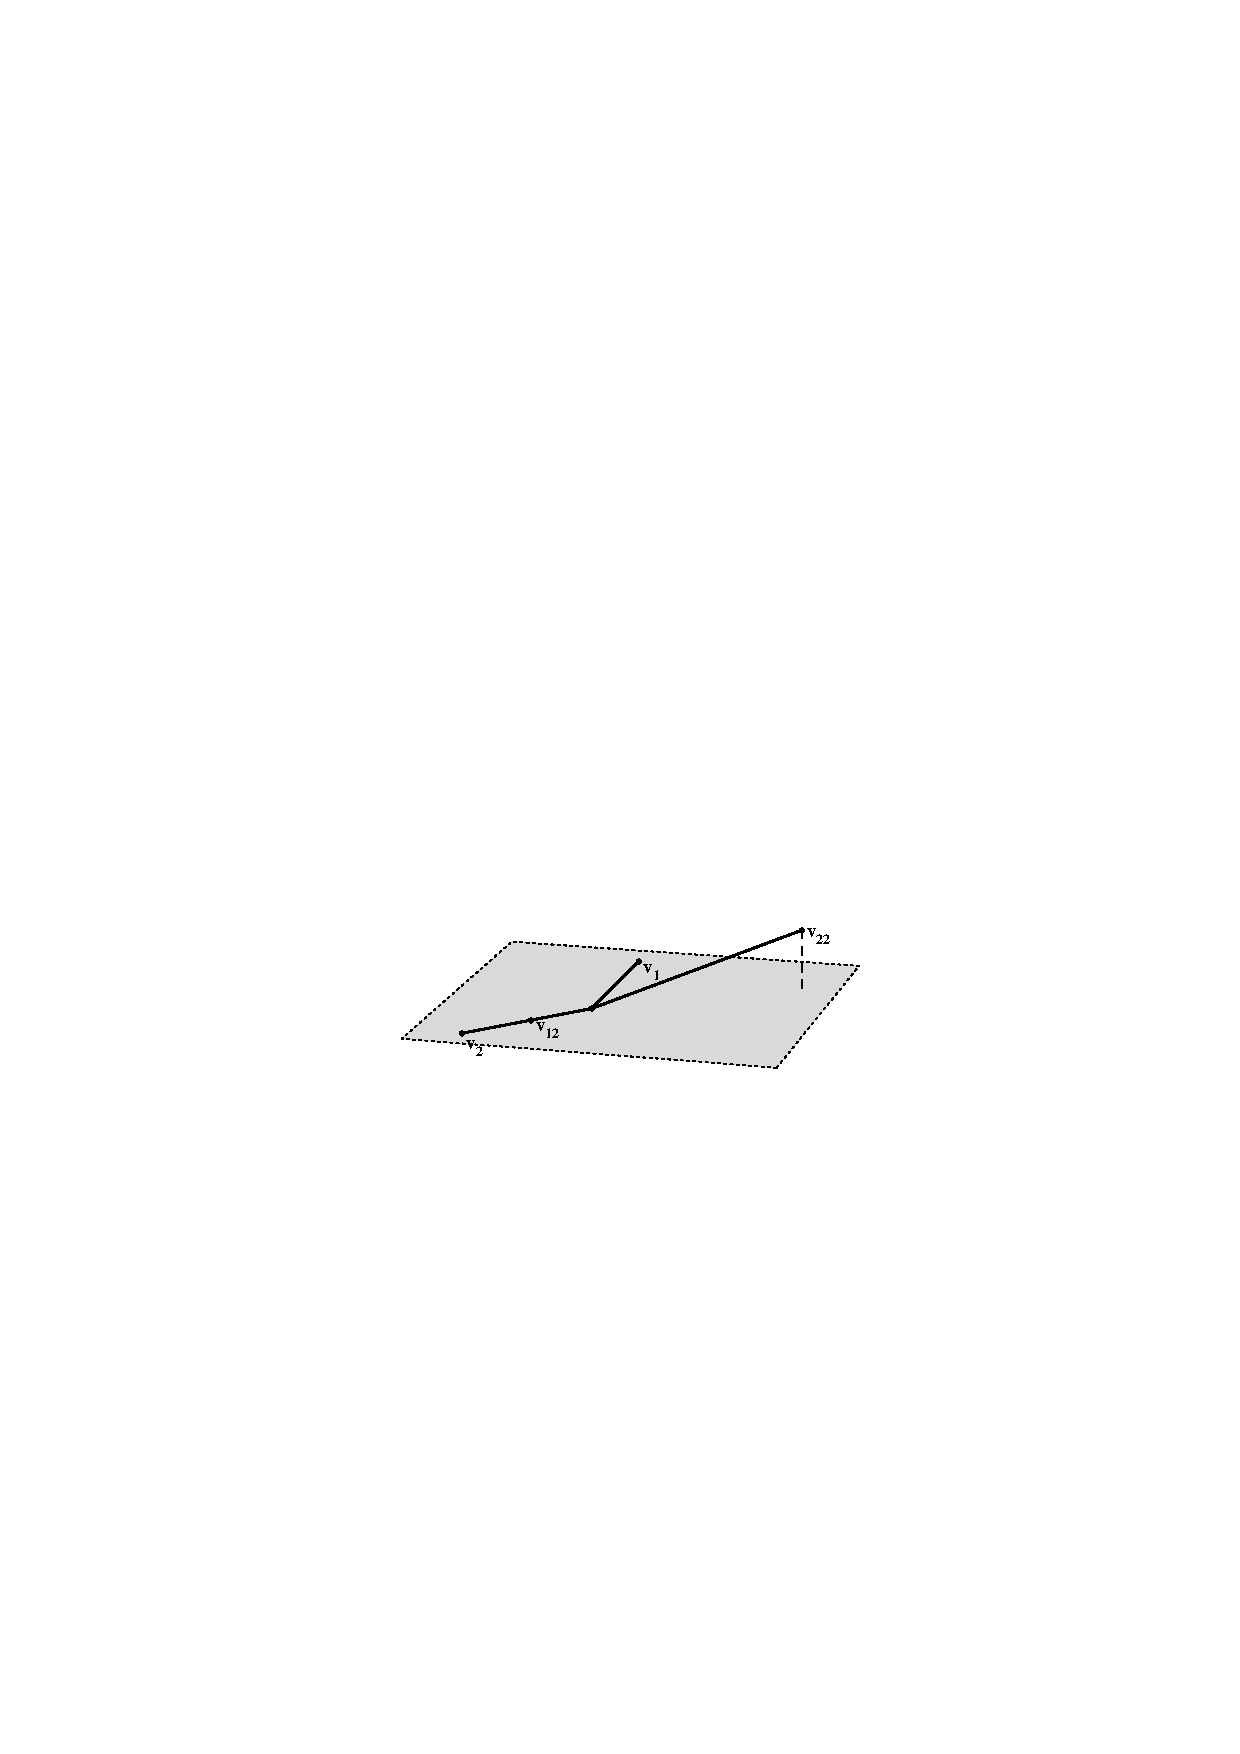
\includegraphics{7PURtanvec}}%,height=3in}}
  \caption{\label{fig:PURtanvec}
  Projection of the scaled velocity and acceleration vectors for the
  Puromycin data at $\hat \btheta=(212.7,0.0641) \trans$ in the
  3-dimensional space spanned by these vectors.  The tangent plane is
  shaded.  }
\end{figure}
we show the projection of the tangent vectors and the acceleration
vectors into the combined tangent and acceleration space
for the Puromycin data.
To provide a clearer figure, we have scaled the response by
dividing by 100 and scaled the concentrations by multiplying by 10.
Note that only the vector $\ddot{\bv}_{22}$ has a component
outside the tangent plane, and that this component is small.
\end{example}

To determine the tangential and normal components of an acceleration
vector, we project the acceleration vectors into the tangent plane and
into the space normal to the tangent space but spanned by the
acceleration vectors.
This is easily accomplished by gathering the $P ( P + 1 ) / 2 $
nonredundant acceleration vectors into a matrix $\ddot{\bW}$ and
combining them with the tangent vectors in $\dot \bV$ to give
\begin{equation}
  \bD = ( \dot{\bV} , \ddot{\bW})
  \label{eqn:boldd}
\end{equation}
We then perform a $QR$ decomposition on $\bD$, as
$\bD=( \bQ_1 | \bQ '_1 | \bQ_2 ) \bR$,
\index{QR decomposition!of velocity and acceleration matrix}
and multiply the array $\ddot{\bV}$ by
$( \bQ_1 | \bQ '_1 ) \trans$ to give
\begin{equation}
  \ddot{\bA} = [ ( \bQ_1 | \bQ '_1 ) \trans ] [ \ddot{\bV}]
  \label{eqn:bolda}
\end{equation}
where $\bQ_1 $ is the first $P$
columns of $\bQ$ and $\bQ '_1 $ is the next $P'$ columns of $\bQ$.
This provides a compact $( P + P' ) \times P \times P$
{\em acceleration array\/} $\ddot{\bA}$ with $P$ faces in the
\index{acceleration!array}
\index{array!acceleration}
tangent space and $P'$ faces in the acceleration space.
(The square bracket notation indicates that the summation is over the
numerator index:
that is, the element in the $n$th face,
$p$th row, and $q$th column of the
product $ \bA = [ \bB ][ \bC ]$, where $\bB$ is an
$N_1 \times N_{2}$
matrix and $\bC$ is an $N_2 \times N_3 \times N_{4}$ array, is
$$
\lb \bA \rb_{npq} = \sum_{i=1}^{ N_2 } { \lb \bB \rb_{ni}
\lb \bC \rb_{ipq} }
$$
and $ \bA $ is an $N_1 \times N_3 \times N_4 $ array.)

\begin{example}\label{mic:adotdot}

To illustrate these calculations, we use the velocity and
acceleration vectors from Example Puromycin~\ref{mic:11}, Table 7.1,
to form the matrix $\bD$.
Performing a $QR$ decomposition on $\bD$ gives
\begin{eqnarray*}
  \bR_1&=&[ ( \bQ_1 | \bQ '_1 ) \trans ] [ \bD ] =
  \left[ \matrix {
  \matrix { \bR_{11} \cr  {\bf 0}  }
  \matrix { \bR_{12} \cr \bR_{22} } }
  \right]\\
  &=&
  \left[ \matrix {
  \matrix { -2.44 \cr 0 \cr 0 }
  \matrix { 1568.7 \cr 1320.3 \cr 0 }
  \matrix { 0 \cr 0 \cr 0 }
  \matrix {  7.378 \cr 6.210 \cr 0 }
  \matrix { -16185.7 \cr -25030.4 \cr 8369.1 } }
  \right]
\end{eqnarray*}
The left upper $2\times2$ matrix, $\bR_{11} $, is simply $\hat{\bR}_{1}$
from the $QR$ decomposition of $\dot \bV$ (cf. Example Puromycin 7),
and the right upper $2\times3$ matrix, $\bR_{12} $, gives the
projection of the acceleration vectors into the tangent plane,
$ [ \bQ_1 \trans ] [ \ddot{\bW}] $.
The $1\times3$ lower right matrix, $\bR_{22}$, gives the
projection of that part of the acceleration vector which is orthogonal
to the tangent space but in the space spanned by the acceleration
vectors, $[ {\bQ_1'}\trans ] [ \ddot{\bW}] $.
In this example, this extra space has dimension $P' = 1 $.

Reforming the elements of $\bR_{12}$ and $\bR_{22}$
into a $3\times2\times2$ acceleration array $\ddot{\bA}$ gives
$$
\ddot{\bA} = \left[ \matrix {
  \matrix { 0 \cr 7.378 }
  \matrix { 7.378 \cr -16185.7 } }
\right]
  \left[ \matrix {
  \matrix { 0 \cr 6.210 }
  \matrix { 6.210 \cr -25030.4 } }
\right]
  \left[ \matrix {
  \matrix { 0 \cr 0 }
  \matrix { 0  \cr 8369.1 } }
\right]
$$
These are the values which, when scaled as in Example Puromycin~\ref{mic:12}, were
used to generate Figure~\ref{fig:PURtanvec}.
\end{example}

The extent to which the acceleration vectors lie outside the
tangent plane measures how much the expectation surface deviates
from a plane, and hence measures the nonplanarity
of the expectation surface.
We call this nonplanarity {\em intrinsic nonlinearity\/} because,
\index{intrinsic!nonlinearity}
\index{nonlinearity!intrinsic}
as discussed in Chapter 2, it does not depend on the
parametrization chosen for the expectation function, but
only on the design and the expression for the expectation function.
The projections of the acceleration vectors in the tangent plane
necessarily depend on the parametrization, and measure the
nonuniformity of the parameter lines on the tangent plane.
This nonuniformity is called {\em parameter effects\/} nonlinearity
or, more simply, {\em parameter effects}.
\index{nonlinearity!parameter effects}
\index{parameter!nonlinearity}
\index{parameter effects!nonlinearity}

Because the elements in the array $\ddot{\bA}$ provide information on the
parameter effects and intrinsic nonlinearities, we write the first $P$
faces of $\ddot{\bA}$ as $\bA^{\theta}$, to denote the parameter effects
acceleration array, and the last $P'$ faces as $\bA^{iota}$, to
denote the intrinsic acceleration array.

\begin{example}\label{rum:7}

In Figure \ref{fig:RUM2expsurf}$a$
\begin{figure}
  \centerline{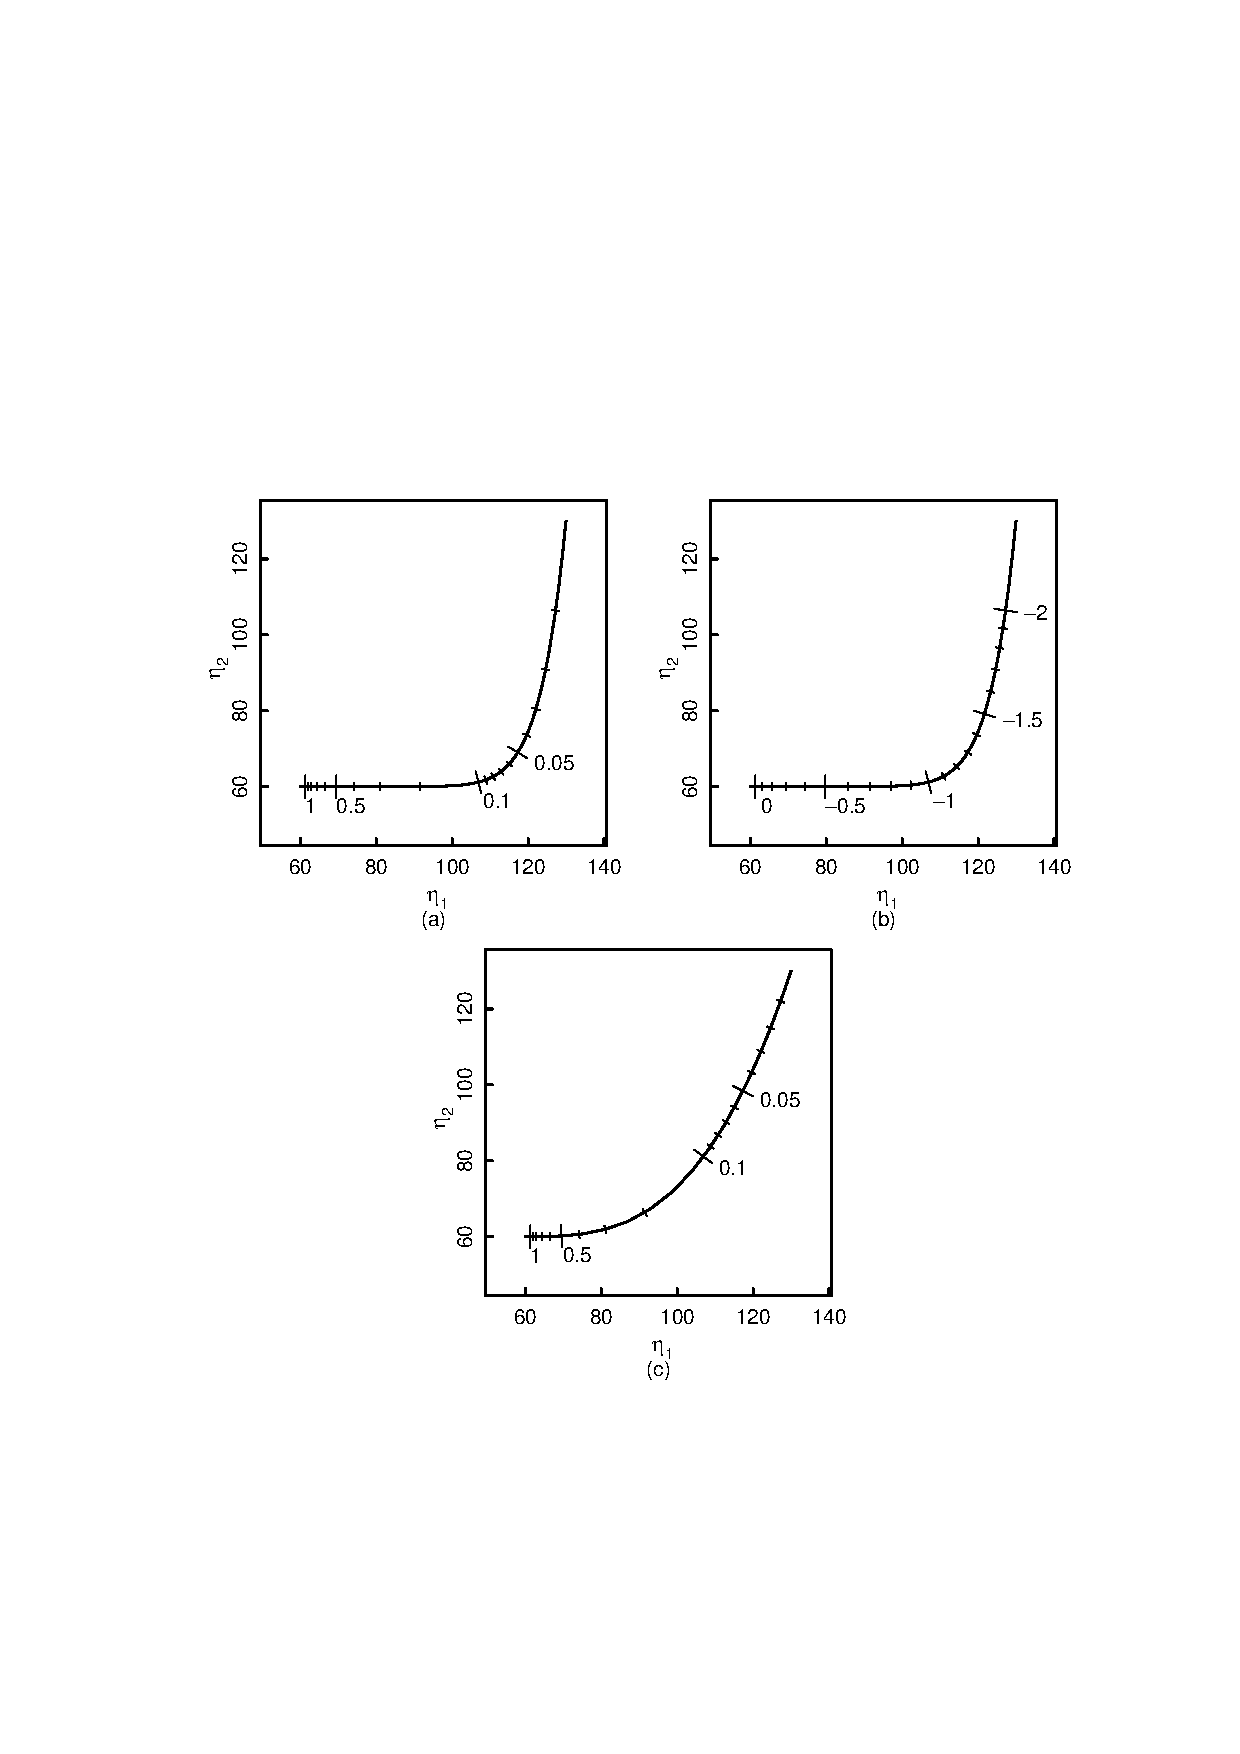
\includegraphics{7RUM2expsurf}}%,height=4in}}
  \caption{\label{fig:RUM2expsurf}
  Plot of the expectation surface (curve) for the 2-case Rumford
  example.  In part $a$, the design is $(4 , 41 ) \trans$'-1p' and the
  parameter is the original parameter $\theta$.  In part $b$, the same
  design is used but the parameter is $\phi=\log_{10} \theta $.  In part
  $c$, the original parameter $\theta$ is used, but the design is
  changed to $(4 , 12 ) \trans$.  }
\end{figure}
we show the expectation surface (curve) $\boeta ( \theta )$
for the Rumford model with the design $\bx=( 4,41) \trans$ and
the parametrization
$$
f=60+70e^{ - x\theta }
$$
The marks on the expectation curve correspond to
$$
\theta=0.01 ,0.02 ,\ldots,0.08 ,0.1 ,0.2 ,\ldots,0.9 ,1.0
$$
and as pointed out in Chapter 2, equally spaced
values of $\theta$ map to unequally spaced values on $\boeta$.
This is a manifestation of the parameter effects nonlinearity,
while the curving of the line is a manifestation of
intrinsic nonlinearity.

In Figure~\ref{fig:RUM2expsurf}$b$ we show the expectation surface
$\boeta ( \phi )$ for the Rumford model with the same design and the
reparametrization $\phi=\log_{10} \theta $,
$$
f=60+70\exp ( - x 10^{\phi} )
$$
The marks on the expectation curve correspond to the values
$$
\phi=-2.0 ,-1.9 ,-1.8 ,\ldots,-0.1 ,0
$$
so that the same range of $\theta$ is covered.
Note that the expectation curves are identical, and that the only
change is a relabeling of the points on the curve.
It is because the curve does not change with the parametrization
that we call the nonlinearity {\em intrinsic}.
Note, too, that points which are equally spaced in the $\phi$
space still map to unequally spaced points on the expectation
curve, but the nonuniformity in the spacing on $\boeta$ is not as
severe as it was for the $\theta$ parametrization.
The $\phi$ parametrization is therefore said to have smaller
parameter effects nonlinearity.

In Figure~\ref{fig:RUM2expsurf}$c$ we show the expectation surface
$\boeta ( \theta )$
for the Rumford model with the $\theta$ parametrization and the
design $\bx = ( 4,  12 ) \trans$.
The main feature to notice is that the expectation surface is
different from that in Figure~\ref{fig:RUM2expsurf}$a$ and
$b$ because the design has been changed.
\end{example}

Reparametrizing a model not only affects the mapping of the parameter
\index{reparametrization!and parameter effects}
lines to the expectation surface but also the tangent and acceleration
vectors, and consequently the parameter effects nonlinearity.

\begin{example}\label{rum:7a}

Shown in Figure~\ref{fig:RUM2derivs}
\begin{figure}
  \centerline{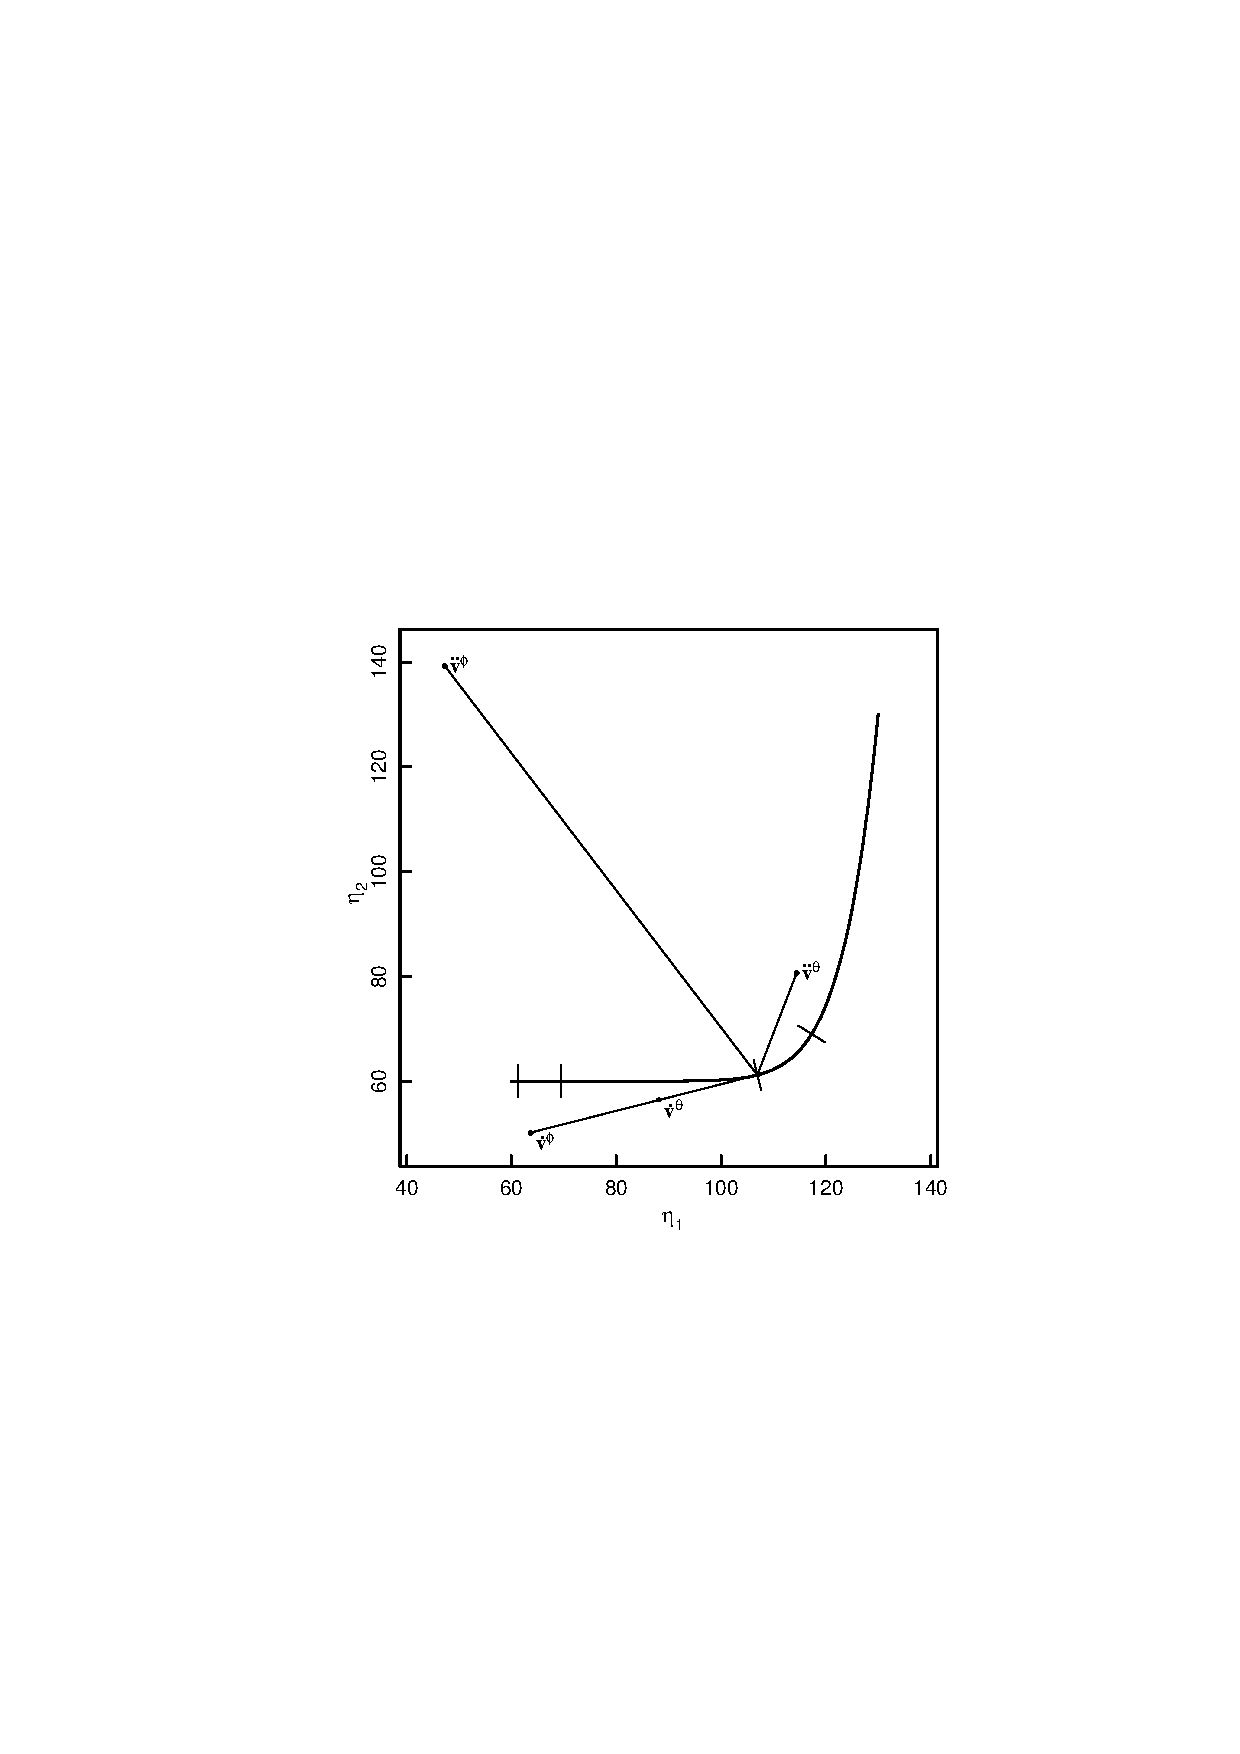
\includegraphics{7RUM2derivs}}%,height=3in}}
  \caption{\label{fig:RUM2derivs}
  Scaled velocity and acceleration vectors at $\theta=1$ for the
  2-case Rumford example using the parameter $\theta$ and the parameter
  $\phi=\log_{10} \theta $.  }
\end{figure}
are the expectation
surface and the acceleration and the tangent vectors at a point on
the surface.
As in Example Puromycin~\ref{mic:12}, we have scaled the parameters and
the design variable to provide a clearer figure.
The design variable is scaled by 0.1, and the parameter $\theta$ by
10.
In this scaling, the point is
$\theta = 1.0$ $( \phi = 0.0 )$ for the $( 0.4,4.1 ) \trans$ design,
corresponding to
$\theta = 0.1$ $( \phi = -1.0 )$ for the $( 4,  41 ) \trans$ design
in the original scaling.

Note that the tangent vectors are in the same direction, as they
must be for them both to be tangent to the same curve.
The {\em lengths\/} of the tangent vectors are very different, however,
and the acceleration vectors are different not only in length,
but also in orientation.
Both these differences are due to the reparametrization, and so
we see some of the effects of parameter nonlinearity.
\end{example}

\subsection{The Acceleration in an Arbitrary Direction}

The velocity and acceleration vectors only provide information
about the expectation surface corresponding to changes along the
parameter axes in the parameter space.
To measure the velocity and acceleration near $\hat{\btheta}$ in an
\index{acceleration!in an arbitrary direction}
arbitrary direction $\bu$ in the parameter space, we introduce a
distance parameter $b$ and let $\btheta = \hat{\btheta}+ b \bu$,
where $\bu$ is a $P \times 1$ unit vector.
Mapping the line $\btheta (b) = \hat{\btheta}+ b \bu$ to the
expectation surface generates a curve
$\boeta_{\bu} (b) = \boeta ( \hat{\btheta} + b \bu )$
through the point $\boeta ( \hat{\btheta} )$.
The tangent and acceleration vector to that curve at $\hat \btheta$
are obtained by differentiating with respect to $b$ and
evaluating the derivatives at $b = 0$.
Thus,
\begin{eqnarray*}
  \left. {{d \boeta_{\bu} \over d b}} \right|_0&=& \sum_{p=1}^P \left.
  {\partial \boeta \over \partial \theta_p} \right|_{\hat {\theta}}
  \left. {d \theta_p \over d b} \right|_0\\
  &=&\sum_{p=1}^P \dot{\bv}_p u_p
\end{eqnarray*}
or, more compactly,
\begin{equation}
  \dot{\boeta}_{\bu}=\dot{\bV}\bu
  \label{eqn:8.3}
\end{equation}
Similarly, the acceleration vector corresponding to the direction
$\bu$ is
\begin{eqnarray}
  \left. {d^2 \boeta_{\bu} \over d b^2} \right|_0&=& \sum_{q=1}^P
  \left.  { \partial { \sum_{p=1}^P { \dot \bv_p u_p}}
  \over
  \partial \theta_q} \right|_{\hat\theta} \left.  { d \theta_q \over d
  b} \right|_0\\
  \label{eqn:8.4a}
  &=& \sum_{p=1}^P \sum_{q=1}^P \ddot \bv_{pq} u_p u_q\nonumber
\end{eqnarray}
which can also be written compactly as
\begin{equation}
  \ddot{\boeta}_{\bu} = \bu \trans \ddot{\bV}\bu
  \label{eqn:8.4}
\end{equation}

From (\ref{eqn:8.3}) we see that
the velocity corresponding to the direction $\bu$ is just a linear
combination of the velocity vectors
$\dot \bv$, and from (\ref{eqn:8.4a}) and (\ref{eqn:8.4})
that the acceleration is also
just a linear combination of the acceleration vectors $\ddot \bv$.
In (\ref{eqn:8.4}), the $N \times1$ vector $\ddot{\boeta}_{\bu}$ is formed
by pre- and postmultiplying the
$N \times P \times P$ array by a $1\times P$ and a $P\times 1$
vector.
Each coordinate of $\ddot{\boeta}_{\bu}$ is of the form
$\bu \trans \ddot \bV_n \bu$, where $\ddot \bV_{n}$ is
the $n $th face of the array $\ddot \bV$.

Since our primary interests are accelerations in and normal to the
tangent plane, we can represent them more compactly by reducing
$\ddot \bV $ to $\ddot{\bA}$ as in (\ref{eqn:bolda}).
In this case, the acceleration corresponding to the direction $\bu$
becomes
\begin{equation}
  \bQ \trans \ddot{\boeta}_{\bu} = \bu \trans \ddot{\bA}\bu
  \label{eqn:8.41}
\end{equation}
or

\begin{equation}
  \bQ \trans \ddot{\boeta}_{\bu} = \sum_{p=1}^{P} \sum_{q=1}^P\lb \ddot
  \bA \rb_{pq} u_p u_q
  \label{eqn:8.42}  
\end{equation}
where $\lb \ddot \bA \rb_{pq} $ is the $(P + P') \times1 $ vector
in the array $\ddot \bA $.
Note that these are simply columns from the matrix $\bR_{1}$ from the $QR$
decomposition of $\bD$, equation (\ref{eqn:boldd}).
Writing the matrix
\begin{equation}
  \left[ \matrix { \matrix {\bR_{12} \cr \bR_{22} } } \right] = \left[
  \matrix { \matrix { \br_{11} , \br_{12} , \br_{22} ,\ldots, \br_{PP}}
  }\right]
  \label{eqn:boldr2}
\end{equation}
then (\ref{eqn:8.42}) can be expressed as
\begin{equation} 
  \bQ \trans \ddot{\boeta}_{\bu} = \sum_{p=1}^P { \br_{pp} u_p^2 } + 2
  \sum_{p=1}^P \sum_{q=p+1}^P \br_{pq} u_p u_q
  \label{eqn:8.43}
\end{equation}
which is a convenient form for calculation.

\begin{example}\label{mic:13}

To illustrate the calculations involved in (\ref{eqn:8.43}),
we calculate the acceleration corresponding to the direction
$\bu  = (0.6 , 0.8 ) \trans$.
Using (\ref{eqn:8.43}) and the values in $\bR_{1}$ from
Example Puromycin \ref{mic:adotdot},
\begin{eqnarray*}  
  \bQ \trans \ddot{\boeta}_{\bu}&=&(0.6)^2 \br_{11} + (0.8)^2
  \br_{22} + 2(0.6)(0.8) \br_{12}\\
  &=&0.36 \left[ \matrix { \matrix { 0
  \cr 0 \cr 0 } } \right] + 0.64 \left[ \matrix { \matrix { -16185.7 \cr
  -25030.4 \cr 8369.1 } } \right] + 0.96 \left[ \matrix { \matrix {
  7.378 \cr 6.210 \cr 0 } } \right]\\
  &=&\left[ \matrix { \matrix { -10351.8 \cr -16013.5 \cr 5356.2 } }
  \right]
\end{eqnarray*}
\end{example}

\section{Relative Curvatures}
\index{relative curvature}

Although accelerations are indicators of nonlinearity, they are
not useful measures of it, because they depend on scaling of the
data and the parameters.
In the Rumford example, for instance, measuring the temperature
on the Celsius instead of the Farenheit scale, or measuring the time
in hours instead of minutes, would produce different
accelerations.
To avoid this dependence, we convert the accelerations to
{\em relative curvatures}.

The {\em curvature\/} $c_{\bu}$ in the direction $\bu$ at a point
\index{curvature!definition}
is defined as the ratio of the length of the acceleration vector
to the squared length of the tangent vector,
$$
c_{\bu} = { \norm \ddot{\boeta}_{\bu} \norm  
\over  \norm \dot{\boeta}_{\bu} \norm^2 }
$$
For parameter effects curvature, we have
\index{parameter effects!curvature}
\index{curvature!parameter effects}
\begin{equation}
  c_{\bu}^{\theta} = { \norm \ddot{\boeta}_{\bu}^{\theta} \norm \over
  \norm \dot{\boeta}_{\bu} \norm^2 }
  \label{eqn:8.7}  
\end{equation}
and for intrinsic curvature,
\index{intrinsic!curvature}
\index{curvature!intrinsic}
\begin{equation}
  c_{\bu}^{iota} = { \norm \ddot{\boeta}_{\bu}^{iota} \norm \over
  \norm \dot{\boeta}_{\bu} \norm^2 }
  \label{eqn:8.6}
\end{equation}

Multiplying the acceleration and tangent vectors by $\bQ \trans$
does not change the magnitude of either the denominator or the numerator,
and so we use the more compact array $\bA^{\theta} $ to
calculate the numerator in (\ref{eqn:8.7}) using
$$
\norm \bu \trans \bA^{\theta} \bu \norm^2 = \sum_{ p = 1 }^P
{ ( \bu \trans \ddot \bA_p \bu )^2 }
$$
and the numerator in (\ref{eqn:8.6}) using
$$
\norm \bu \trans \bA^{iota} \bu \norm^2 =
\sum_{ p = P + 1 }^{ P + P' }
{ ( \bu \trans \ddot \bA_p \bu )^2 }
$$
The denominators are calculated using
\begin{eqnarray*}
  \norm \dot{\boeta}_{\bu} \norm^2&=&\norm \dot \bV \bu \norm^2\\  
  &=&\bu \trans \bR_{11} \trans \bR_{11} \bu\\
  &=&\norm \bR_{11} \bu \norm^2
\end{eqnarray*}
where $\bR_{11}$ is from the $QR$ decomposition of $\bD$, (\ref{eqn:boldd}).

To simplify calculation of the curvatures, we arrange that
$\norm \dot{\boeta}_{\bu} \norm^{2}=1$
for any $\bu$ with $\norm \bu \norm = 1 $ by
linearly tranforming to orthogonal parameters
\begin{equation}
  \bphi = \bR_{11} ( \btheta - \hat \btheta )
  \label{eqn:8.6c}
\end{equation}
Furthermore, since curvatures are measured in units of 1/response,
their values depend on the scaling of the data.
To remove this dependence,
we convert to dimensionless {\em relative curvatures\/} by
multiplying the response and the curvatures by $s \sqrt{P}$.
The final result is a {\em relative curvature array\/}
\index{relative curvature!array}
\index{array!relative curvature}
\begin{equation}
  \bC = \bR_{11} \invtrans \ddot \bA \bR_{11}^{-1} s \sqrt{P}
  \label{eqn:relcurveq}
\end{equation}
which consists of a $P \times P \times P$
{\em parameter effects relative curvature array\/}
$\bC^{\theta}$,
\index{parameter effects!relative curvature array}
given by the first $P$ faces of $\bC$ and a $P' \times P \times P$
{\em intrinsic relative curvature array\/} $\bC^{iota}$, given by the
\index{intrinsic!relative curvature array}
last $P'$ faces of $\bC$.

An important consequence of scaling by $s \sqrt{P}$ is that the
sum of squares contour bounding a nominal $1 - \alpha$
likelihood region on the tangent plane is simply
\index{likelihood!region, scaled}
a disk of radius $\sqrt{\FPNP}$, and the
likelihood region itself, determined from (6.1), becomes all values
of $\btheta$ for which the (scaled) sum of squares equals
$1+[ P / ( N -P) ] \FPNP$.
This affords a convenient scale of measurement for the curvatures.

\begin{example}\label{mic:15}

For the Puromycin data, $s = 10.93$, $P = 2 $,
$$
\bR_{11}^{-1} = \left[ \matrix {
  \matrix { -0.4092 \cr 0 }
  \matrix { 0.4861 \cr 0.0007574 } }
\right]
$$
and, from Example Puromycin~\ref{mic:adotdot},
$$
\ddot \bA = \left[ \matrix {
  \matrix { 0 \cr 7.378 }
  \matrix { 7.378 \cr -16185.7 } }
\right]
  \left[ \matrix {
  \matrix { 0 \cr 6.210 }
  \matrix { 6.210 \cr -25030.4 } }
\right]
  \left[ \matrix {
  \matrix { 0 \cr 0 }
  \matrix { 0  \cr 8369.1 } }
\right]
$$
so that
$$
\bC =
\left[ \matrix {
\matrix {0.000 \cr } \matrix {-0.035 \cr -0.059} }\right]
\left[ \matrix {
\matrix {0.000 \cr } \matrix {-0.030 \cr -0.151} }\right]
\left[ \matrix {
\matrix {0.000 \cr } \matrix {0.000 \cr 0.074} }\right]
$$
where the first two matrices give $\bC^{\theta}$, and the
third, $\bC^{iota}$.
Since each face of $\bC$ is symmetric, we only display the upper
triangular part; for example, in the above array,
$c_{212} = -0.030 = c_{221} $.

Because the curvatures are small, we expect that the tangent
plane would provide a good approximation to the expectation
surface and that projections of the parameter curves on the tangent
plane would be quite uniform.
In Figure~\ref{fig:PURphitau}$a$
\begin{figure}
  \centerline{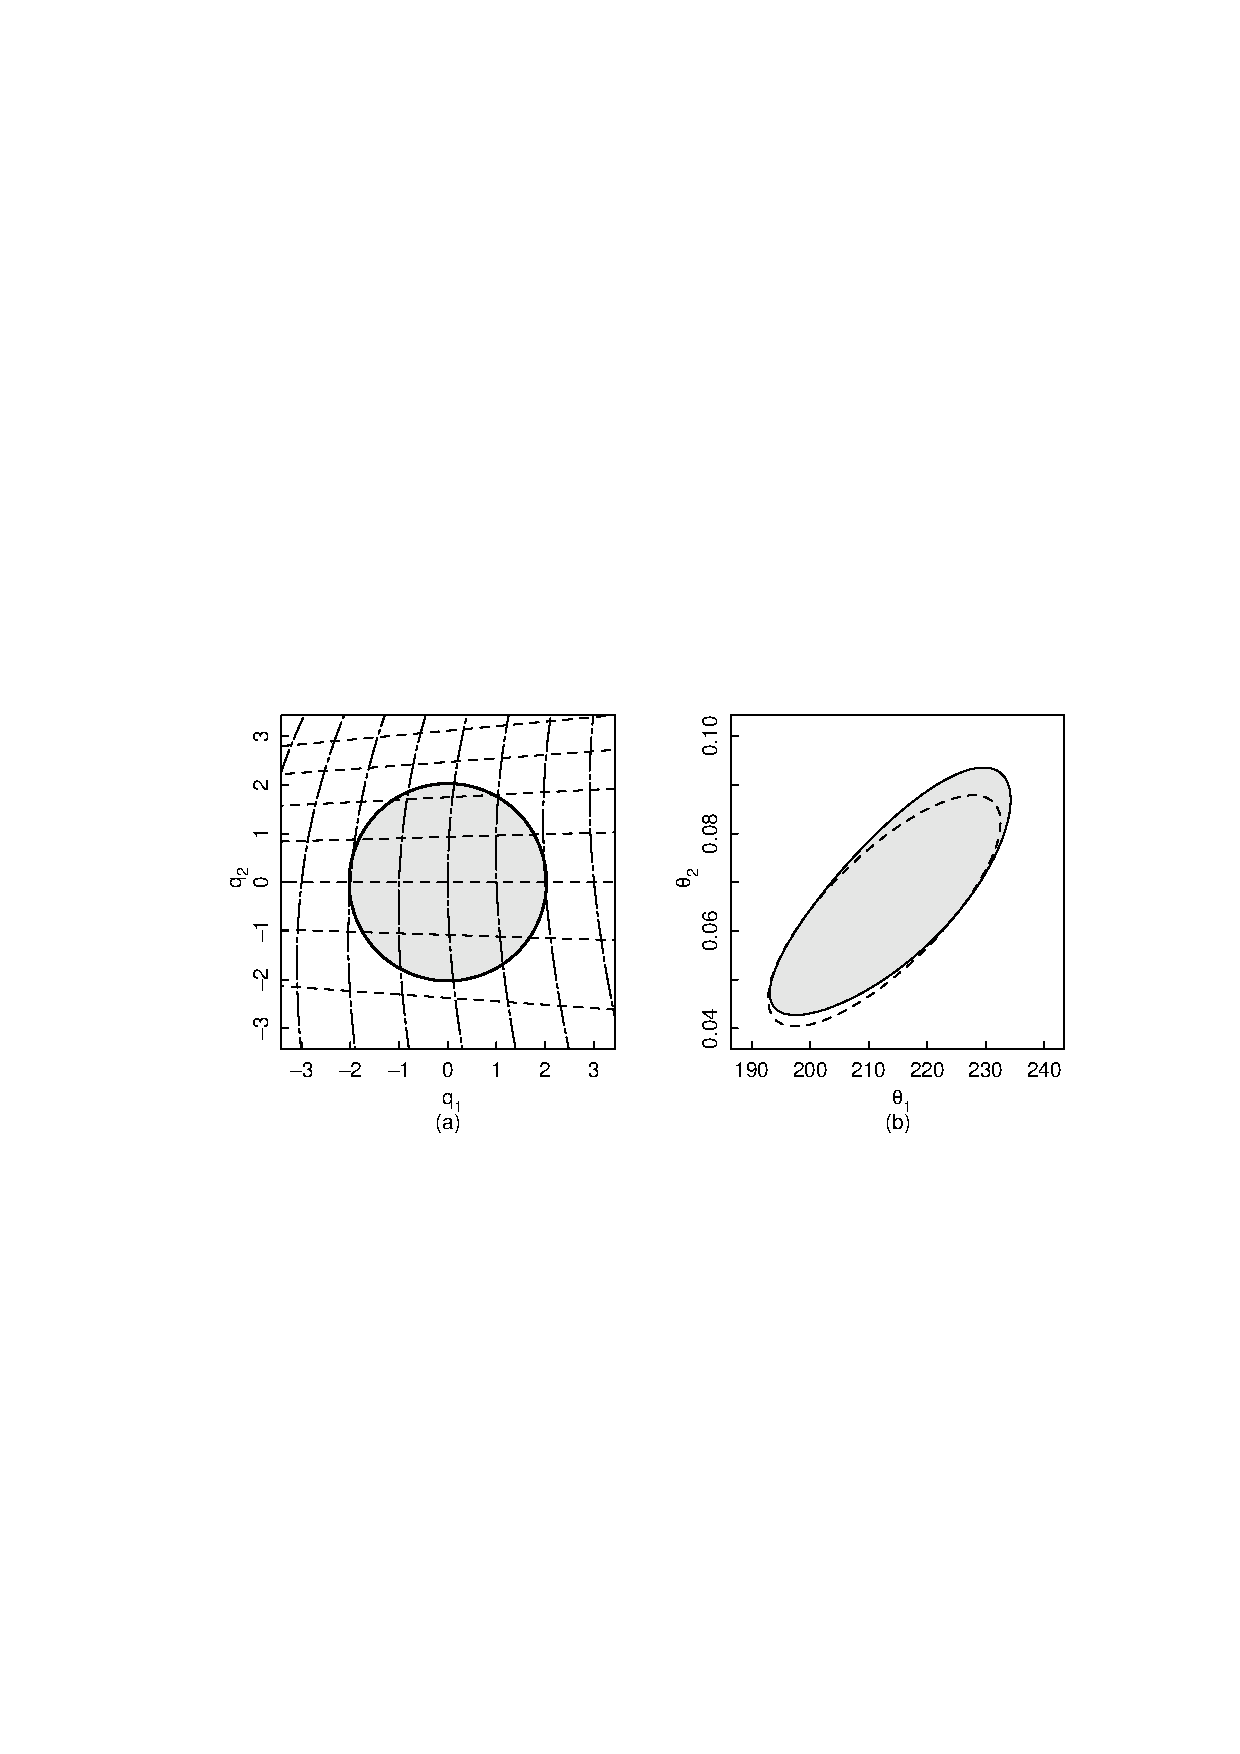
\includegraphics{7PURphitau}}%,height=2.25in}}
  \caption{\label{fig:PURphitau}
  Likelihood regions for the parameters in the Puromycin model.  In
  part $a$, the parameter curves for the parameters $\phi=\bR_{11} (
  \btheta - \hat \btheta )$ are projected onto the tangent plane with
  the 95\% likelihood disk, assuming the expectation surface is planar,
  shaded.  In part $b$, this region is transformed to the $\btheta$
  parameter space and shaded.  The ellipse shown as a dashed line in
  part $b$ is from the linear approximation.  }
\end{figure}
we show projections of the $\bphi$ parameter curves on the tangent
plane.
As expected, the curves are quite straight, parallel, and equispaced.

Also shown in Figure~\ref{fig:PURphitau}$a$ is the
tangent plane disk of radius
$\sqrt { F( 2, 10;  0.05 ) } = 2.02$.
Since the region is not too large, the parameter curves are well
behaved within it and we would expect a linear approximation
region to give a good approximation to the true likelihood
region.
This is indeed the case, as demonstrated in Figure \ref{fig:PURphitau}$b$,
where we
show the linear approximation region (dashed line) and the
likelihood region (solid line) determined from the (scaled) sum of
squares contour $S( \btheta ) = 1 + ( 2 / 10) 4.10 = 1.82$.
\end{example}

The relative curvature array $\bC$ is not unique, since any
transformation to orthogonal parameters $\bphi$ could be
used, and any orthogonal rotation of the response space
could be used, provided the tangent and its orthogonal are
kept distinct.
The parameter transformation given by $\bR_{11}$ is convenient.

An algorithm for calculating the relative curvature array was presented
\index{relative curvature!algorithm}
in \citeasnoun{bate:hami:watt:1983}.
%\glossary{ Bates, D.M.}
%\glossary{ Hamilton, D.C.}
%\glossary{ Watts, D.G.}
They combine $\dot \bV$ and the nonredundant
$\ddot \bV$ vectors into a matrix $\bD$, the first $P$ columns of
which contain the first derivative vectors $\dot \bv_{p}$ and the
remaining $P( P + 1)/2$ columns the second derivative vectors
$\ddot \bv_{pq}$ stored in symmetric storage mode; that is, in
the order $11,12, 22, 13 ,..., PP$.
They then use a pivoted $QR$ decomposition \cite[Chapter 9]{dong:bunc:mole:stew:1979}
%\glossary{ Dongerra, J.J.}
%\glossary{ Bunch, J.R.}
%\glossary{ Moler, C.B.}
%\glossary{Stewart, G.W.}
to write $\bD = \bQ \bR \bE$, where $\bQ$ is $N \times N$ orthogonal,
$\bE$ is a $P( P + 3)/2$ square permutation matrix in which the
upper left $P \times P$ submatrix is the identity, and $\bR$ is upper
trapezoidal with the upper-left $P \times P$ submatrix being upper
triangular.
They assume $\dot \bV$ is nonsingular but do not require $\bD$ to be so.

Partitioning $\bR$ as
$$
\bR = \left[ \matrix {
\matrix { \bR_{11} \cr  {\bf 0}  \cr  {\bf 0}  }
\matrix { \bR_{12} \cr \bR_{22}  \cr  {\bf 0}  }
}\right]
$$
provides $\bR_{11}$, which is used to produce $\bphi$,
$\bR_{12}$, which is used to produce $\bC^{\theta}$, and
$\bR_{22}$, which is used to produce $\bC^{iota}$.
The number of nonzero rows in $\bR$ is the dimension of the
combined tangent and acceleration spaces.
The first $P$ columns of $\bQ$, $\bQ_{1}$, form an orthogonal
basis for the tangent space and the next $P'$ columns, ${\bQ}_{1}'$,
form an orthogonal basis for the normal acceleration space.

To calculate the curvature arrays, each $P \times P$ face of the
3-dimensional array formed by expanding the second derivative
columns from the symmetric storage mode must be postmultiplied by
$\bR_{11}^{-1}$ and premultiplied by
$\bR_{11}^{{-} {\rm T}}$.
These two multiplications are replaced by a single
postmultiplication of the last $P( P + 1)/2$ columns of $\bR$ by
a matrix composed of products of elements of
$\bR_{11} \trans$, which creates the symmetric storage
version of the curvature array with dimension
$(P + P') \times P ( P - 1 ) / 2 $
\cite{bate:hami:watt:1983}.
%\glossary{ Bates, D.M.}
%\glossary{ Hamilton, D.C.}
%\glossary{ Watts, D.G.}
This {\em relative curvature matrix\/} gives a more compact representation
of the
\index{relative curvature!matrix}
\index{matrix!relative curvature}
curvatures, with the first  $P$ rows revealing the parameter
effect relative curvature terms and the last $P'$ rows the
intrinsic curvature terms.
Alternatively, each column gives a curvature vector for a particular
parameter pair.

\begin{example}\label{mic:15mat}

From Example Puromycin~\ref{mic:15}, the curvature matrix is
$$
\left[ \matrix {
  \matrix { 0 \cr 0 \cr 0 }
  \matrix { -0.035 \cr -0.030 \cr 0 }
  \matrix { -0.059 \cr -0.151 \cr 0.074 } }
\right]
$$
For this model and data set, all the relative curvatures are
small, and so the estimation situation is probably not badly affected
by the nonlinearity.
\end{example}

\subsection{Interpreting Terms in the Curvature Arrays}
\subsubsection{Intrinsic Curvatures}

The geometric interpretation of intrinsic curvature is that it is
\index{intrinsic curvature!geometric interpretation}
the reciprocal of the radius of the circle which best approximates
the expectation surface in the direction $\boeta_{\bu}$.
Thus, if the planar assumption is good, the intrinsic curvature will be
small.
\index{assumptions!planar}
\index{planar assumption!and intrinsic curvature}

\begin{example}\label{rum:8}

In Figure~\ref{fig:RUM2curv}
\begin{figure}
  \centerline{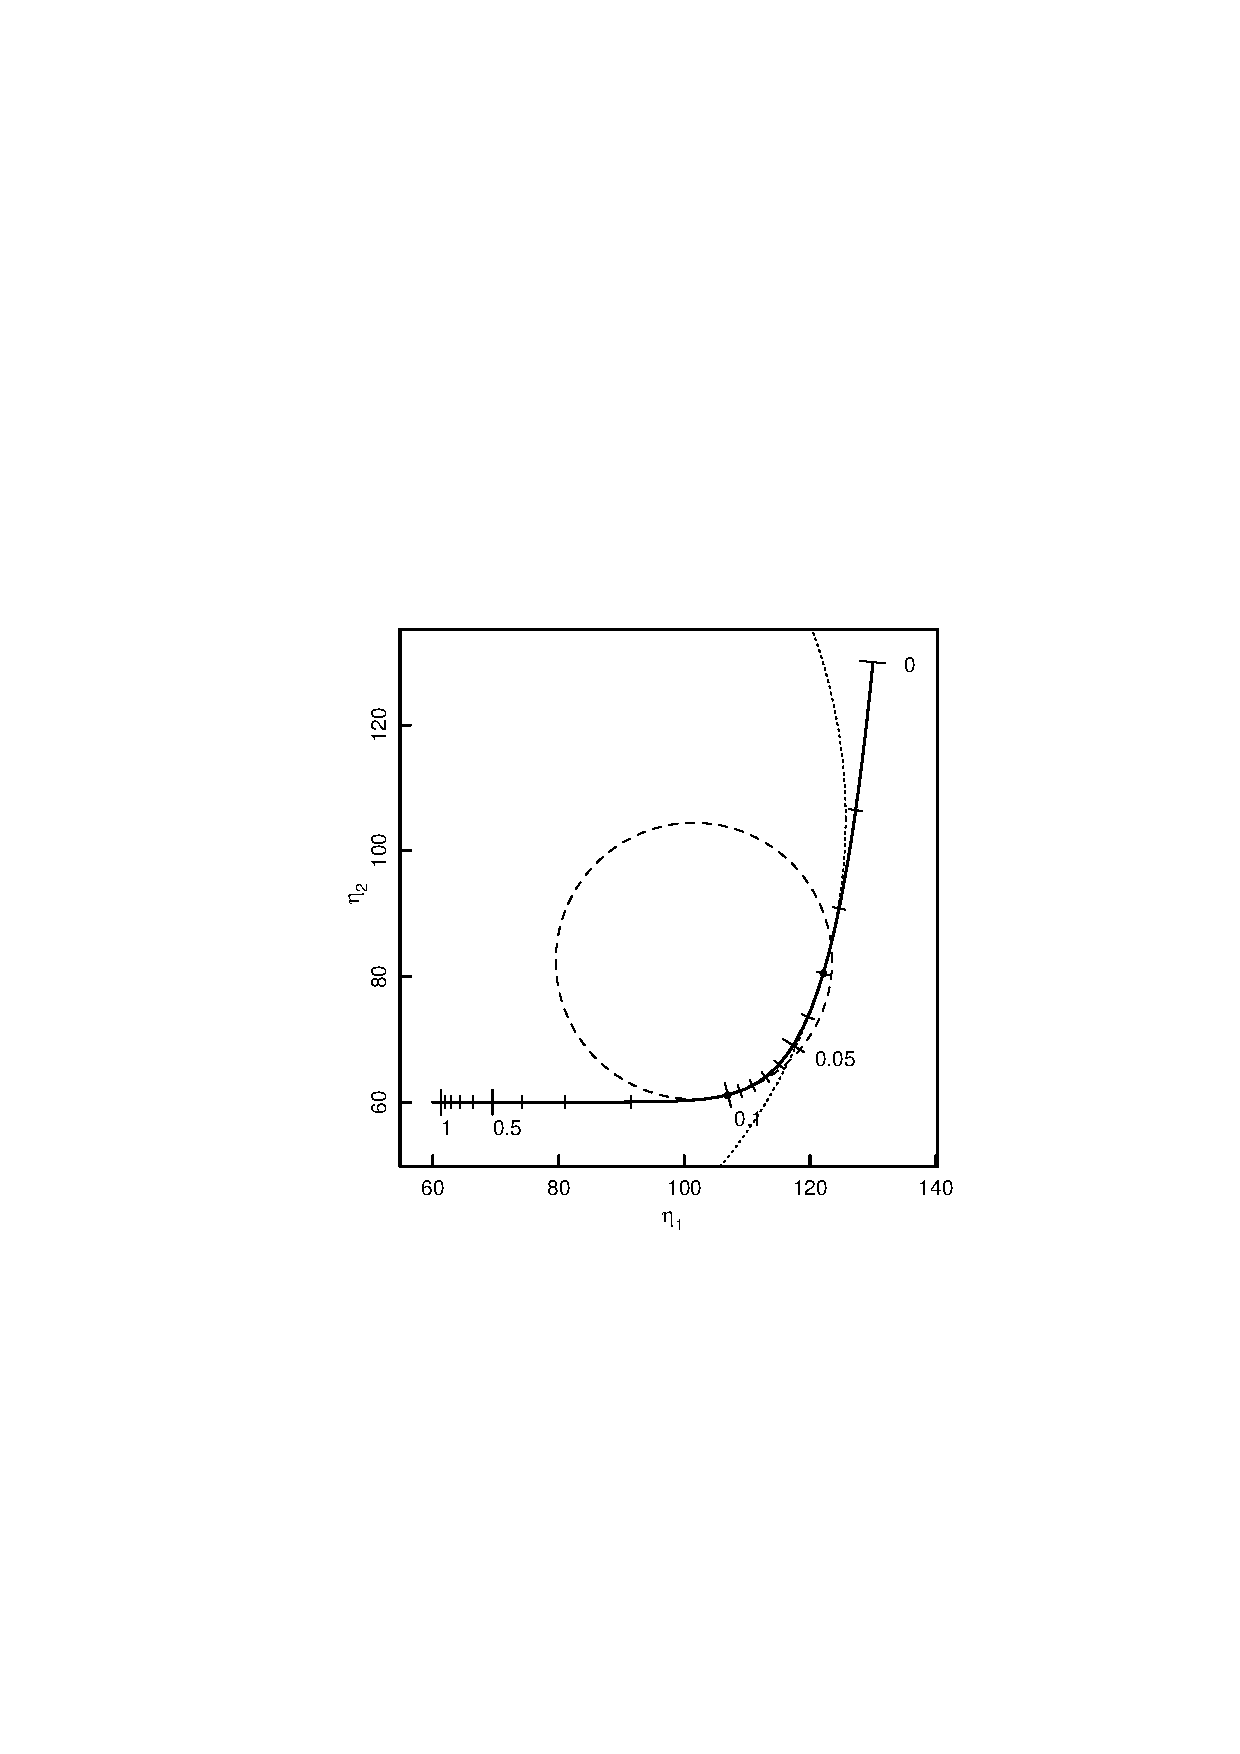
\includegraphics{7RUM2curv}}%,height=3in}}
  \caption{\label{fig:RUM2curv}
  Approximating circles to the expectation surface for the 2-case
  Rumford example.  The dashed circle is the approximation to the
  surface based on the intrinsic curvature at $\theta=0.1$.  The dotted
  circle is the approximation to the surface based on the intrinsic
  curvature at $\theta=0.03$.  }
\end{figure}
we show the expectation curve for the Rumford
model with the design $\bx = ( 4,  41 ) \trans$, together with portions
of the approximating circles at points corresponding to
$\theta = 0.1$ and $\theta = 0.03$.
For $\theta = 0.1$ the circle has a curvature of
$1706 / 37490 = 0.046$ with a radius of
$1 / 0.046 = 22$, and for $\theta = 0.03$ the
larger circle has a curvature 0.0115 with a radius of
$1 / 0.0115 = 87$.
\end{example}

\begin{example}\label{mic:15a}

In Figure \ref{fig:PURphisurf}
\begin{figure}
  \centerline{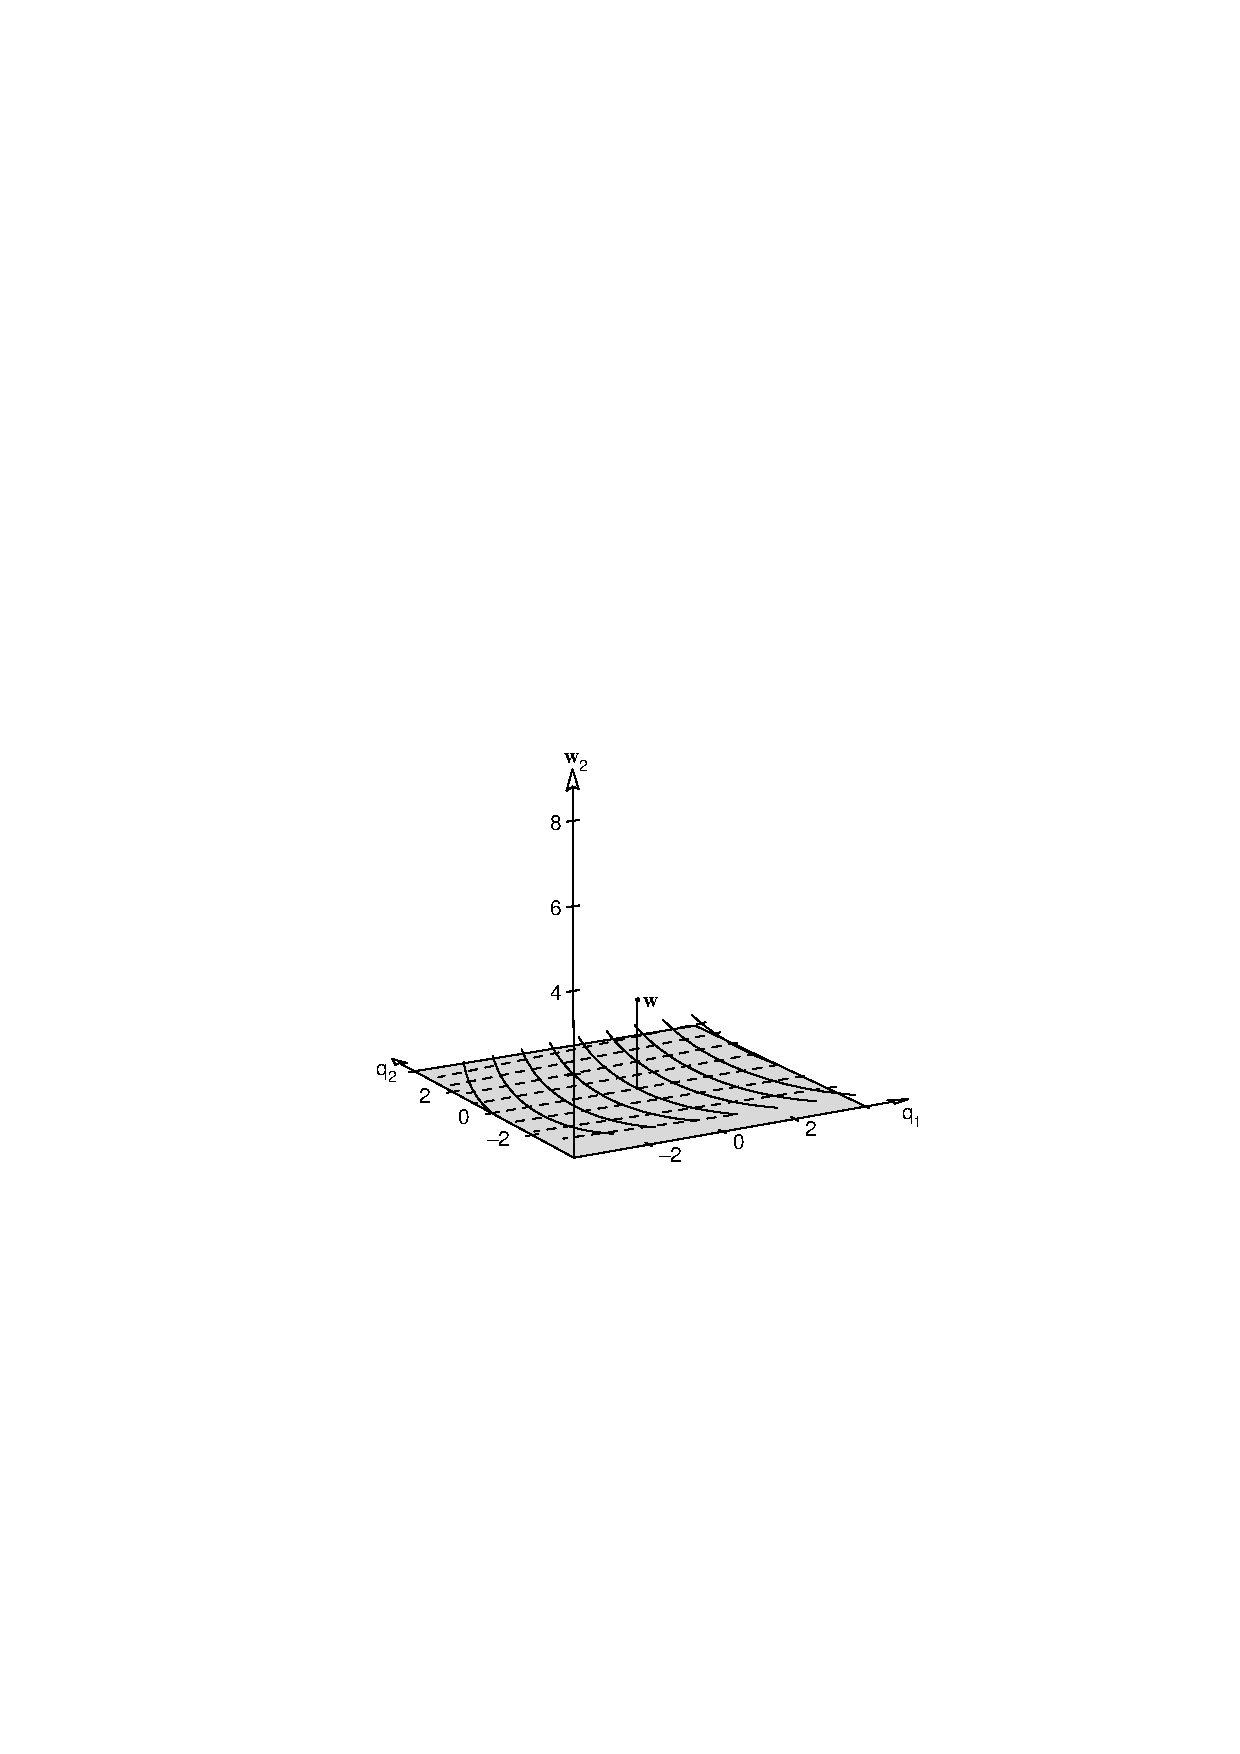
\includegraphics{7PURphisurf}}%,height=3in}}
  \caption{\label{fig:PURphisurf}
  Projection of the parameter curves from the orthogonal parameters
  $\bphi=\bR_{11} ( \btheta - \hat \btheta )$ for the Puromycin data
  model into the 3-dimensional subspace spanned by the tangent plane
  vectors, $\bq_{1}$ and $\bq_{2}$, and the rotated residual vector,
  $\bw$.  The tangent plane is shaded.  }
\end{figure}
we show the expectation surface in the space spanned by the tangent
vectors and the residual vector for the Puromycin data.
The surface is extremely flat, and so the tangent plane provides an
excellent approximation to the expectation surface near $\hat \btheta$.
This is expected, given the magnitudes of the entries in the
intrinsic curvature array
$$
\bC^{iota} =
\left[ \matrix {
\matrix {0.000 \cr } \matrix { 0.000  \cr  0.074} }\right]
$$
\end{example}

\subsubsection{Parameter Effects Curvatures}

Each of the terms $c_{npq} $ in the relative curvature
array has a geometric interpretation, which helps in
\index{parameter effects!curvature - geometric interpretation}
understanding nonlinearity \cite{bate:watt:1981:anna}.
%\glossary{ Bates, D.M.}
%\glossary{ Watts, D.G.}
To interpret the terms $c_{npq}$, we consider a 2-parameter
example.

The tangential components of the scaled velocity and acceleration
vectors evaluated at $\bphi =  {\bf 0} $ are
\begin{eqnarray*}
  \dot\bv_1(\bphi={\bf 0})&=&\bq_1\\
  \dot\bv_2(\bphi={\bf 0})&=&\bq_2\\
\end{eqnarray*}
and
\begin{eqnarray*}
  \ddot \bv_{11}&=&c_{111} \bq_1 + c_{211} \bq_2\\
  \ddot \bv_{12}&=&c_{112} \bq_1 + c_{212} \bq_2\\
  \ddot \bv_{22}&=&c_{122} \bq_1 + c_{222} \bq_2  
\end{eqnarray*}
At another point $\bphi = \bdelta$ the new tangent vectors will
be approximately
\begin{eqnarray*}
  \dot \bv_1 ( \bdelta )&\approx&
  \dot \bv_1 (  {\bf 0}  ) +
  \delta_1 \left. { \partial \dot \bv_1   \over  \partial \phi_1 }
  \right|_{{\phi} =  {\bf 0}  } + 
  \delta_2 \left. { \partial \dot \bv_1   \over  \partial \phi_2 }
  \right|_{{\phi} =  {\bf 0}  }\\
  &=&\bq_1 + \delta_1 \ddot \bv_{11} +\delta_2 \ddot \bv_{12}
\end{eqnarray*}
and
$$
\dot \bv_2 ( \bdelta )  \approx
\bq_2 + \delta_1 \ddot \bv_{21} +
\delta_2 \ddot \bv_{22}
$$
Collecting terms in $\bq_{1}$ and $\bq_{2}$ gives
\begin{eqnarray*}
  \dot \bv_1 ( \bdelta )&=&
  \bq_1 ( 1 +
  \delta_1 c_{111} + \delta_2 c_{112} ) +
  \bq_2 ( \delta_1 c_{211} + \delta_2 c_{212} )\\
  \dot \bv_2 ( \bdelta )&=&
  \bq_1 ( \delta_1 c_{112} + \delta_2 c_{122} ) +
  \bq_2 (1 + \delta_1 c_{212} + \delta_2 c_{222} )
\end{eqnarray*}
Thus, $c_{111}$ gives the change in the $\bq_{1}$ direction of
the $\dot \bv_{1}$ vector due to a unit change in $\phi_{1}$:
that is, terms of the form $c_{ppp}$ cause the vector
$\dot \bv_{p}$ to change length.
We therefore refer to $c_{ppp}$ as {\em compansion\/} terms since
\index{parameter!compansion}
\index{compansion}
they cause compression or expansion of scale along a $\phi_{p}$
parameter line.
The term $c_{211}$ gives the change in the $\bq_{2}$ direction
of the $\dot \bv_{1}$ vector due to a unit change in $\phi_{1}$:
that is, terms of the form $c_{qpp} ( q != p )$ cause changes
in the $\bq_{q}$ direction of the $\phi_{p}$ parameter lines as
we move along them.
We refer to these as {\em arcing\/} terms.
\index{parameter!arcing}
\index{arcing}
The term $c_{212}$ gives the change in the $\bq_{2}$ direction
of the $\dot \bv_{2}$ vector due to a unit change in $\phi_{1}$:
that is, terms of the form $c_{qpq}$ cause changes in the
$\bq_{q}$ direction of the $\phi_{p}$ parameter curves as we
move across the $\phi_{q}$ parameter curves.
We call these {\em fanning\/} terms, since the $\phi_{p}$ parameter
\index{parameter!fanning}
\index{fanning}
lines will appear to fan out from a common point on the
$\bq_{p}$ axis.
Since $c_{qqp} = c_{qpq}$, terms of the form $c_{qqp}$
also cause $\phi_{p}$ fanning.

With two parameters, only compansion, arcing, and fanning can
occur;  with more than two parameters, only one more type of
parameter effect can occur---when all the subscripts are
different.
A term such as $c_{npq}$ causes a change in the $\bq_{n}$
direction of the $\dot \bv_{p}$ tangent vector due to a unit
change in $\phi_{q}$.
We refer to these as {\em torsion\/} terms, since they cause a
\index{parameter!torsion}
\index{torsion}
twisting of the $( \phi_p , \phi_q )$ parameter surface,
where a parameter surface---analogous to a parameter curve---is
the set of points generated by holding all $\phi_{p}$'s except
two constant and varying those two.

The interpretation of the individual elements in $\bC$ also helps to
interpret the parameter effects curvature in a particular
direction.
For a direction $\bu$ which is parallel to a parameter axis,
$c_{\bu}^{\theta}$ is the square root of the sum of squares of
the compansion term and all the arcing terms for that parameter.
This is also the case for a general $\bu$:  $c_{\bu}^{\theta}$
measures a combination of the arcing and compansion in the
direction $\bu$.
\label{bod:4}
\begin{example}

For the BOD data, the parameter effects curvature array is
$$
\bC^{\theta} =
\left[ \matrix {
\matrix {0.000 \cr } \matrix {-0.157 \cr 2.100} }\right]
\left[ \matrix {
\matrix {0.000 \cr } \matrix {-0.096 \cr 0.497} }\right]
$$
Examination of the terms in $\bC^{\theta}$ reveals the following:
\begin{enumerate}
\item the $\phi_{2}$ parameter lines will be perfectly uniformly
  spaced along the $\phi_{1}$ lines, since the $\phi_{1}$ term $c_{111}$
  is zero;
  
\item the $\phi_{1}$ parameter curves will be markedly nonuniformly
  spaced along the $\phi_{2}$ lines, since the $\phi_{2}$ compansion
  term $c_{222}$ is large (0.497);
  
\item the $\phi_{2}$ parameter lines will be markedly curved, because
  the $\phi_{1}$ arcing term $c_{122}$ is extremely large (2.100);
  
\item the $\phi_{1}$ parameter lines will be straight, because the
  $\phi_{2}$ arcing term $c_{211}$ is zero;
  
\item the $\phi_{2}$ parameter lines will show modest fanning, because
  the $\phi_{1}$ fanning term $c_{121} = c_{112}$ is quite small
  (--0.157);
  
\item the $\phi_{1}$ parameter lines will show modest fanning, because
  the $\phi_{2}$ fanning term $c_{221} = c_{212}$ is quite small
  (--0.096).
  
\end{enumerate}

In Figure~\ref{fig:BODphitau} 
\begin{figure}
  \centerline{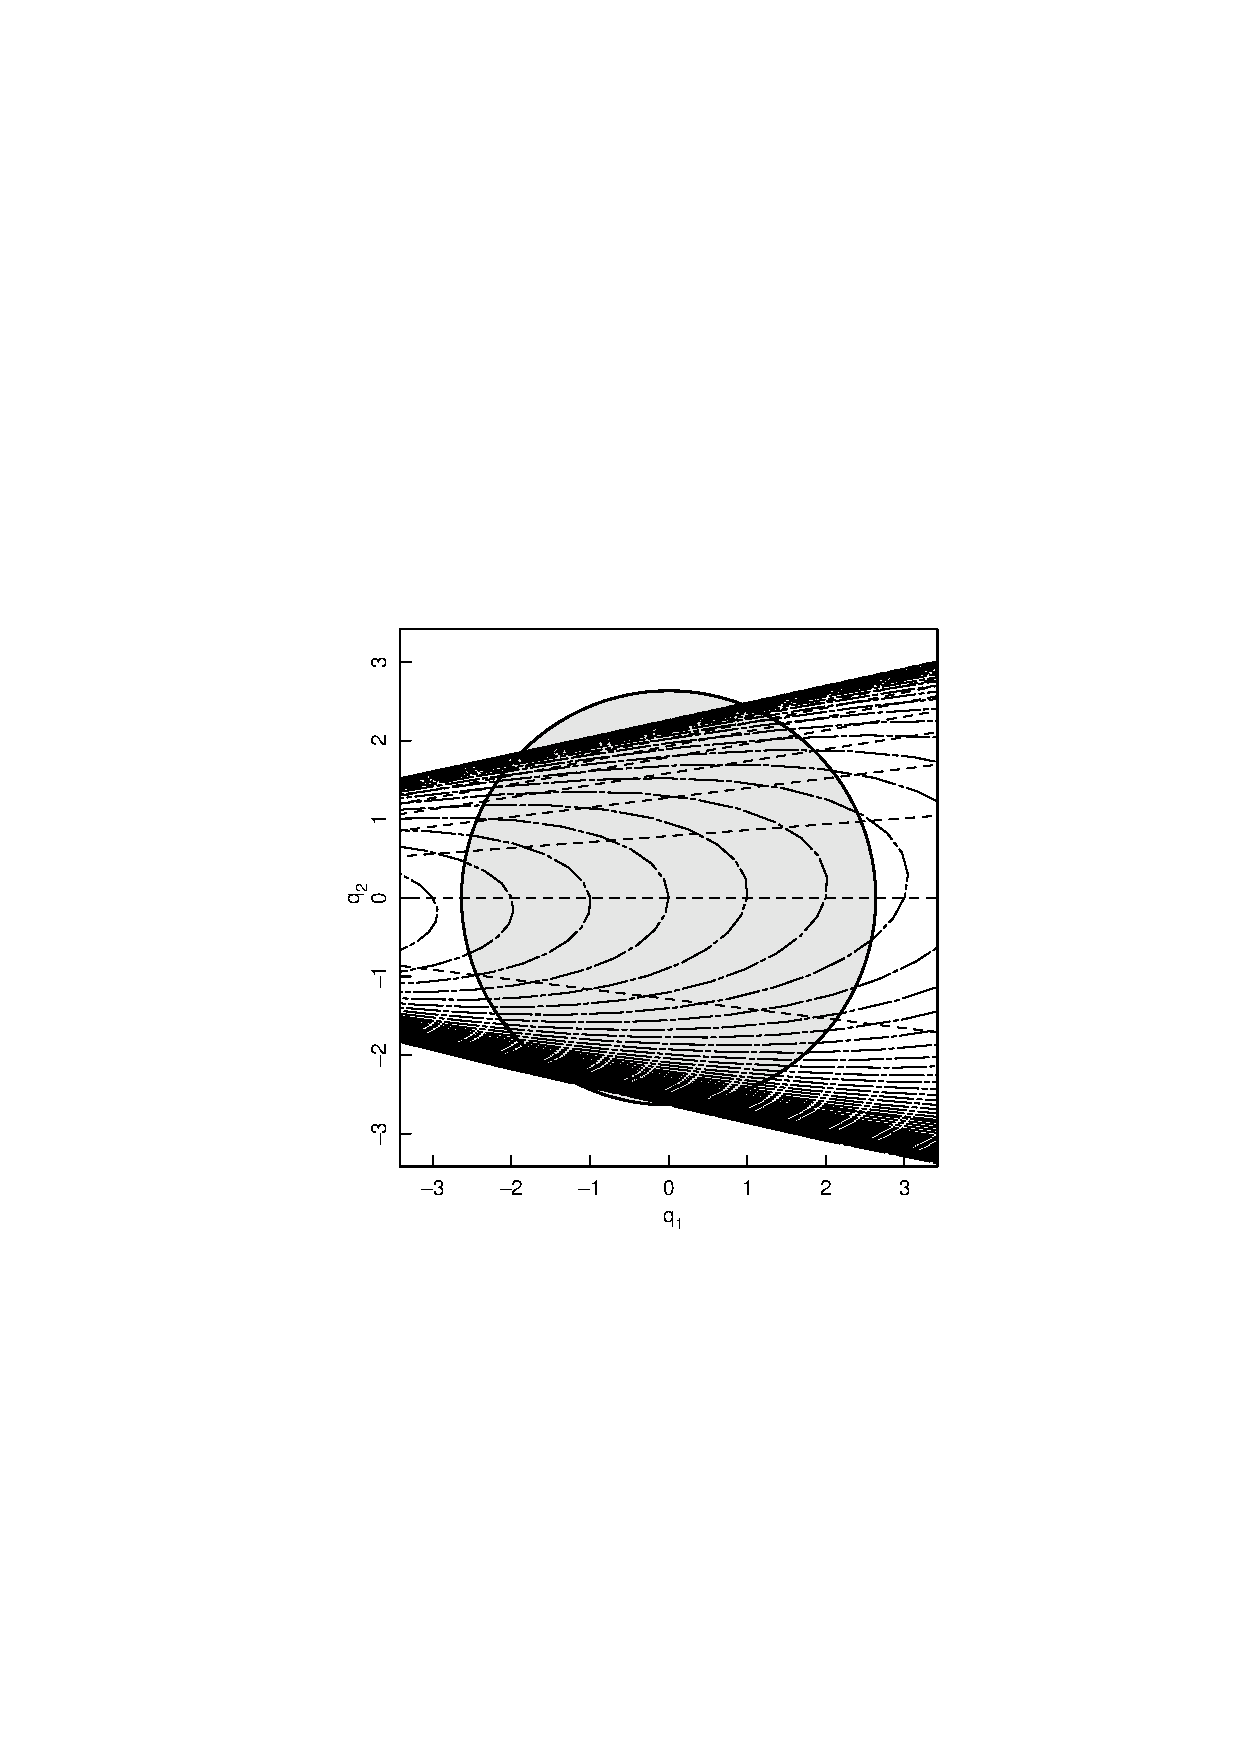
\includegraphics{7BODphitau}}%,height=3in}}
  \caption{\label{fig:BODphitau}
  Parameter curves for the orthogonal parameters $\phi=\bR_{11} (
  \btheta - \hat \btheta )$ for the BOD data.  The parameter curves are
  projected onto the tangent plane, and the circular region
  corresponding to a 95\% likelihood contour (assuming the expectation
  surface is planar) is shaded.  The parameter curves for $\phi_{1}$ are
  indicated by short dashes, and the $\phi_{2}$ parameter curves by
  long--short dashes.  }
\end{figure}
we show the BOD parameter curves projected onto
the tangent plane.
We recall that a parameter curve is associated with the
parameter which is varying, so the short dash curves, corresponding
to fixed $\phi_{2}$, are actually $\phi_{1}$ parameter curves,
and the long--short dash curves, corresponding to fixed $\phi_{1}$,
are actually $\phi_{2}$ parameter curves.
Thus by referring to Figure \ref{fig:BODphitau}, we can see that the parameter
curves behave in the way predicted.

Note that the 95\% likelihood disk extends beyond the expectation
surface and that linear approximation parameter lines would not
adequately approximate the true parameter curves within the disk.
\end{example}

\subsection{Reparametrization}

In Section 7.1 we saw that a transformation of parameters
can make great changes in the parameter effects
nonlinearity,
and in Chapter 6 we saw that such transformations can
greatly improve profile likelihood plots.
Unfortunately, there is little guidance available as to the
choice of a reparametrization and its effects in a particular
\index{reparametrization}
\index{transformation!of parameters}
\index{parameter!transformation}
situation.
As shown in \citeasnoun{bate:watt:1981:anna} transformations which are
%\glossary{ Bates, D.M.}
%\glossary{ Watts, D.G.}
recommended for certain types of parameters and models can
decrease the parameter effects nonlinearity for one data set and
increase them for another.
Consequently, it may be necessary to experiment with several
transformations to find a suitable one,
as done, for example, in \citeasnoun{ratk:1983}.
%\glossary{ Ratkowsky, D.A.}

It would be tedious to evaluate
parameter transformations by finding the parameter
effects curvature array for a particular
expectation function--data set combination under a
reparametrization by (1) restating the
model in terms of the new parameters, (2) recalculating all the
derivatives, and (3) determining the $\bC$ array.
Fortunately this work can be avoided.

Suppose we wish to determine the parameter effects array,
$\bC^{\beta}$, corresponding to a reparametrization in which the
new parameters $\bbeta$ are nonlinear transformations of $\btheta$,
$$
\bbeta = \bG ( \btheta )
$$
or
$$
\beta_p = \bG_p ( \btheta )  p=1,2 ,..., P
$$
We assume the inverse transformation is
$$
\btheta = \bD ( \bbeta )
$$
or
$$
\theta_p = \bD_p ( \bbeta ) p=1,2 ,..., P
$$
and write the $P \times P$ Jacobian matrices as $\dot \bD$ and
\index{Jacobian!matrix}
$\dot \bG$ with $(n,p)$th elements
${ \partial \bD_n } / { \partial \beta_p } $ and
${ \partial \bG_n } / { \partial \theta_p } $ respectively.

The $P \times P \times P$ second derivative arrays are written as
\index{second derivative!array}
$\ddot \bD$ and $\ddot \bG$ with elements
${ \partial^2 \bD_n } / { \partial \beta_p  \partial \beta_q }$
and
${ \partial^2 \bG_n } / { \partial \theta_p  \partial \theta_q }$
respectively:  a term with subscript $npq$ resides in the
$n $th face, $p $th row, and $q $th column.
[It may be helpful to note that the $n $th row of $\dot \bG$ is
the gradient of $\bG_p $,
$ { \partial \bG_p } / { \partial \btheta \trans } $,
and that the $p $th row of the $n $th face of
$\ddot \bG$ is the gradient of
$ { \partial \bG_n } / { \partial \theta_p } $,
$( \partial /{\partial \btheta \trans})
 \partial \bG_n / \partial \theta_{p}$.]

Using the chain rule for differentiation, the new tangent vectors
at the least squares estimates $ \hat{\bbeta}=\bG(\hat{\btheta})$
are
\begin{eqnarray*}
  \dot\bb_p&=&\left.{\partial \boeta \over \partial \beta_p}
  \right|_{\hat {\beta}}\\
  &=& \sum_{q=1}^P
  \left( \left. { \partial \boeta   \over  \partial \theta_q }
  \right|_{\hat {\theta}}\right) 
  \lb \dot \bD \rb_{qp}\\
 &=&
 \sum_{q=1}^P \dot \bv_q  \lb \dot \bD \rb_{qp}
\end{eqnarray*}
where $\dot\bv_q $ is the $q $th column of $ \dot \bV$.
Equivalently, we have
\begin{eqnarray}
  \dot\bB&=&( \dot \bb_1 , \dot \bb_2 ,..., \dot \bb_P )\\
  &=&\dot \bV \dot \bD\nonumber\\
  &=&\bQ_1 \bR_1 \dot \bD\nonumber
  \label{eqn:8.23}
\end{eqnarray}
Similarly the new second derivative vectors are
\begin{eqnarray*}
  \ddot\bb_{pq}&=&\left.
  { \partial^2 \boeta   \over  \partial \beta_p \partial \beta_q }
  \right|_{\hat {\beta}}\\
  &=&{\partial\over\partial\beta_q}\left(\sum_{r=1}^P\dot \bv_r \lb
  \dot \bD \rb_{rp}\right)\\
  &=&\sum_{r=1}^P \dot \bv_r \lb \ddot \bD \rb_{rpq}  +
  \sum_{r=1}^P\sum_{s=1}^P
  \lb \dot \bD \rb_{rp} \ddot \bv_{rs} \lb \dot \bD \rb_{sq}
\end{eqnarray*}
where $\ddot \bv_{rs}$ is the $(r,s)$th vector in the array
$ \ddot \bV $.
Thus
\begin{equation}
  \ddot \bB = \dot \bD \trans \ddot \bV \dot \bD + [ \dot \bV ][ \ddot
  \bD ]
  \label{eqn:8.24}
\end{equation}
so
$$
\bA^{\beta} = [ \bQ_1 \trans ] [ \ddot \bB ] =
\dot \bD \trans \bA^{\theta} \dot \bD +
[ \bR_1 ] [ \ddot \bD ]
$$
where, again, the square brackets imply that the summation involved in
the multiplication is over the numerator index.
Now
$$
\bC^{\theta} =
\bR_1 \invtrans \bA^{\theta} \bR_1^{-1}
$$
and the equivalent expression for $\bC^{\beta} $ is, from (\ref{eqn:8.23}),
$$
\bC^{\beta} =
( \bR_1 \dot \bD ) \invtrans \bA^{\beta}
( \bR_1 \dot \bD )^{-1}
$$
so
\begin{eqnarray}
  \bC^{\beta}&=&
  ( \bR_1 \dot \bD ) \invtrans [ \bR_1 ] [ \ddot \bD ]
  ( \bR_1 \dot \bD )^{-1} +
  \bR_1 \invtrans \bA^{\theta} \bR_1^{-1}\\
  \label{eqn:8.25}
  &=&
  ( \bR_1 \dot \bD ) \invtrans [ \bR_1 ] [ \ddot \bD ]
  ( \bR_1 \dot \bD )^{-1} +
  \bC^{\theta}\nonumber\\
  &=&
  [ \bR_1 ]
  [ \bR_1 \invtrans \dot \bD \invtrans \ddot \bD
  \dot \bD^{-1} \bR_1^{-1} ] +
  \bC^{\theta}\nonumber\\
  &=&
  - [ \bR_1 ] [ \bR_1 \invtrans \bT \bR_1^{-1} ] +
  \bC^{\theta}\nonumber
\end{eqnarray}
The quantity $\bT$ is called the {\em transformation curvature array},
\index{transformation!curvature array}
\index{array!transformation}
\begin{equation}
  \bT=- \dot \bD \invtrans \ddot \bD \dot \bD^{-1}
  \label{eqn:8.26}
\end{equation}
since it is in the form of a curvature, that is,
acceleration/velocity$^{2}$.

Thus, the array $ \bC^{\beta} $ equals the original array
$\bC^{\theta}$ minus an adjustment,
$$
\bC^{\beta} = \bC^{\theta} -
[ \bR_1 ] [ \bR_1 \invtrans \bT \bR_1^{-1} ]
$$
Now $\bT$ is given in terms of derivatives with respect to $\bbeta$,
and it is more convenient to have it in terms of the
original parameters $\btheta$.
By writing
$$
\bbeta = \bG ( \bD ( \bbeta ) )
$$
and differentiating with respect to $ \bbeta $, we have
$$
{\partial \bbeta   \over  \partial \bbeta \trans } = \bI = \dot \bG \dot \bD
$$
and
$$
{\partial^2 \bbeta   \over  \partial \bbeta \partial \bbeta \trans } =
 {\bf 0}  = \dot \bD \trans \ddot \bG \dot \bD + [ \dot \bG ] [ \ddot \bD ]
$$
and so, from (\ref{eqn:8.26}),
$$
\bT:= [ \dot \bG^{-1} ] [ \ddot \bG ]
$$
Finally, we have the result
\begin{equation}
  \bC^{\beta} = \bC^{\theta} - [ \bR_1 ] [ \bR_1 \invtrans [ \dot
  \bG^{-1} ] [ \ddot \bG ] \bR_1^{-1} ]
  \label{eqn:8.30}
\end{equation}

\begin{example}\label{mic:repar}

The Michaelis--Menten model is a ratio of polynomials, and so, as noted
at the end of Section 6.1.2, reparametrizing in the form
$$
f = {x \over  \beta_1 + \beta_2 x }
$$
should reduce the parameter effects (although for this example, they are
already small).
The reparametrization in this case is
$$
\bbeta = \left[ \matrix {
  \matrix {{{ \theta_2   \over  \theta_1 }} \cr
        { {1 \over  \theta_1 } } }
}\right]
$$
and so
$$
\dot \bG = \left[ \matrix {
  \matrix {
    {{- \theta_2 \over \theta_1^2}}\cr
    {{-1 \over \theta_1^2}}
  }
  \matrix {{1 \over \theta_1} \cr 0}
}\right]
$$
and
$$
\ddot \bG=\left[ \matrix {
  \matrix {
    {{2 \theta_2  \over \theta_1^3}} \cr
    {{-1 \over \theta_1^2}}
  }
  \matrix {{{-1 \over \theta_1^2}} \cr 0}
}\right] 
\left[ \matrix {
  \matrix {{2 \over \theta_1^3} \cr \matrix{ \cr 0}}
  \matrix {0 \cr \matrix{ \cr 0}}
}\right]
$$
The product $\bT = [ \dot \bG^{-1} ] [ \ddot \bG ]$ is then
$$
\bT = \left[ \matrix {
  \matrix {{-2 \over \theta_1} \cr \matrix{ \cr 0}}
  \matrix {0 \cr \matrix{ \cr 0}}
}\right]
\left[ \matrix {
  \matrix {0 \cr {-1 \over \theta_1}}
  \matrix {{-1 \over \theta_1} \cr 0}
}\right]
$$
Finally, substituting the parameter values and
performing the remaining multiplications and subtractions as in
(\ref{eqn:8.30}) gives
\begin{eqnarray*}
  \bC^{\beta}&=&
  \left[ \matrix {
  \matrix {0.000 \cr } \matrix {-0.035 \cr -0.059} }\right]
  \left[ \matrix {
  \matrix {0.000 \cr } \matrix {-0.030 \cr -0.151} }\right]
  -
  \left[ \matrix {
  \matrix {0.000 \cr } \matrix { 0.003 \cr -0.027} }\right]
  \left[ \matrix {
  \matrix {0.000 \cr } \matrix { 0.002 \cr -0.005} }\right]\\
  &=&
  \left[ \matrix {
  \matrix {0.000 \cr } \matrix {-0.038 \cr -0.032} }\right]
  \left[ \matrix {
  \matrix {0.000 \cr } \matrix {-0.032 \cr -0.146} }\right]
\end{eqnarray*}
As expected, the change in the parameter effects is slight.
\end{example}

\begin{example}\label{iso:repar}

For the isomerization data,
$$
\bC^{\theta}=
\left[ \matrix {
\matrix {0.000 \cr  \cr  \cr  }
\matrix {-0.110 \cr -0.064 \cr  \cr  }
\matrix {-0.256 \cr  1.762 \cr 8.180 \cr  }
\matrix { 0.361 \cr -18.157 \cr -48.275 \cr 119.610 }
}\right] 
\left[ \matrix {
\matrix {0.000 \cr  \cr  \cr  }
\matrix { 0.000 \cr  0.013 \cr  \cr  }
\matrix { -0.032 \cr -0.102 \cr 0.413 \cr  }
\matrix { 0.000 \cr  -0.004 \cr -4.919 \cr 0.009 }
}\right] \matrix{
\left[ \matrix {
\matrix {0.000 \cr  \cr  \cr  }
\matrix {-0.032 \cr -0.264 \cr  \cr  }
\matrix { 0.000 \cr  0.269 \cr 0.008 \cr  }
\matrix { 0.000 \cr  -4.898 \cr -0.004 \cr 0.008 }
}\right] \cr
\left[ \matrix {
\matrix {0.000 \cr  \cr  \cr  }
\matrix { 0.000 \cr  0.020 \cr  \cr  }
\matrix { 0.000 \cr -0.004 \cr -0.001 \cr  }
\matrix { -0.032 \cr  -0.102 \cr  0.265 \cr -9.826 }
}\right]}
$$
so that the parameter effects nonlinearities are disastrous.
If we reparametrize using the $\bbeta$ parameters of
Example Isomerization 5, it is clear from the discussion in Chapter 6
that the parameter effects will be reduced to an extremely small amount.
Using the above techniques we find the following parameter effects
array for the $\bbeta$ parameters:
$$
\bC^{\beta}=
\left[ \matrix {
\matrix {-0.069 \cr  \cr  \cr  }
\matrix { 0.011 \cr -0.062 \cr  \cr  }
\matrix {-0.007 \cr  0.001 \cr -0.060 \cr  }
\matrix { 0.006 \cr  0.004 \cr  0.003 \cr -0.052 }
}\right] 
\left[ \matrix {
\matrix {-0.007 \cr  \cr  \cr  }
\matrix { 0.001 \cr -0.016 \cr  \cr  }
\matrix {-0.060 \cr -0.015 \cr 0.018 \cr  }
\matrix { 0.003 \cr  0.005 \cr -0.005 \cr -0.035 }
}\right] \matrix{
\left[ \matrix {
\matrix { 0.011 \cr  \cr  \cr  }
\matrix {-0.062 \cr -0.032 \cr  \cr  }
\matrix { 0.001 \cr -0.016 \cr -0.015 \cr  }
\matrix { 0.004 \cr  0.007 \cr  0.005 \cr -0.039 }
}\right] \cr
\left[ \matrix {
\matrix { 0.006 \cr  \cr  \cr  }
\matrix { 0.004 \cr  0.007 \cr  \cr  }
\matrix { 0.003 \cr  0.005 \cr -0.005 \cr  }
\matrix { -0.052 \cr -0.039 \cr -0.035 \cr -0.088 }
}\right]}
$$

The parameter effects are reduced to negligible values, as
expected from the analysis in Chapter 6.
\end{example}

Two important points should be noted.
First, the transformation curvature array $\bT$ is expressed in terms of
the original parameters $ \btheta $, so we do not have to determine the
inverse transformation.
Second, a new array $ \bC^{\beta} $ is
calculated from the array $\bC^{\theta}$ and the
matrix $\bR_{1}$ from previous calculations, a total of only
${ P^2 ( P + 3 ) } / { 2 }$ values.
Equation (\ref{eqn:8.30}) is therefore an extremely efficient expression
for computing the effect of a transformation.

\section{RMS Curvatures}

An appreciation of the terms in the curvature array is helpful to
understanding nonlinearity, but for data analysis we need a
simple overall measure of nonlinearity so that we can assess
the quality of a linear approximation in a particular situation.
For this purpose, we use the {\em root mean square\/} 
(RMS) curvature which is the square
\index{root mean square (RMS)!curvature}
\index{curvature!root mean square (RMS)}
root of the average over all directions of the squared curvature.
We denote the RMS parameter effects curvature by $c^{\theta}$
and the RMS intrinsic curvature by $c^{iota}$.
Formal expressions for a general RMS curvature are developed
below:  the results for parameter effects or intrinsic curvature
are obtained by simply inserting superscripts $^{\theta}$ and
$^{iota}$ in the resulting equations and selecting the
appropriate range of the index $n$.

\subsection{Calculating RMS Curvatures}

The curvature corresponding to the
direction $\bu$ on the tangent plane is
\begin{eqnarray*}
  c_{\bu}&=&\norm \bu \trans \bC \bu \norm\\
  &=&\sqrt { \sum_n^{}  ( \bu \trans \bC_n \bu )^2 }  
\end{eqnarray*}
where $\bC_{n}$ is the $n $th face of $\bC$.
The mean square curvature is then obtained by integrating
$c_{\bu}^{2}$ over all directions $\bu$ and dividing by the surface
area $A$ of the $P$-dimensional sphere.
That is,
\begin{equation}
  c^2 = { 1 \over A } \int { \sum_n { ( \bu \trans \bC_n \bu )^2
  } d A }
  \label{eqn:8.11}
\end{equation}
where $dA$ is the element of surface area on the sphere.
This integral can be expressed as a sum of integrals, giving the
final result \cite{bate:watt:1980}
%\glossary{ Bates, D.M.}
%\glossary{ Watts, D.G.}
\begin{equation}
  c^2 = { 1 \over P ( P + 2 ) } \sum_n \left[ 2 \sum_{p=1}^P
  \sum_{q=1}^P c_{npq}^2 + \left( \sum_{p=1}^P c_{npp}
  \right)^2\right]
\label{eqn:8.12}
\end{equation}
In (\ref{eqn:8.11}) and (\ref{eqn:8.12}),
the index $n$ goes from 1 to $P$
for $c^{\theta}$ and
from $P + 1$ to at most $P( P + 3 )/2$
for $c^{iota}$.

The mean square curvature for 2-parameter models can be
expressed as a 1-dimensional integral over an angle $\omega$,
since then $\bu = [ \cos\omega ,\sin\omega ] \trans$.
Equation (\ref{eqn:8.11}) then becomes
$$
c^2 = { 1   \over  2 \pi }
\sum_n { \int_0^{{2} \pi} {
\left[ c_{n11} \cos^2 \omega +
2 c_{n12} \sin  \omega  \cos  \omega +
c_{n22} \sin^2 \omega\right]^2 d \omega } }
$$
After expanding the square in the integral, all terms involving
odd powers of sines or cosines integrate to 0.
The remaining integrals contribute the amounts
$\frac{3}{8}c_{n11}^2 $, $\frac{3}{8}c_{n22}^2 $,
$\frac{1}{4}c_{n11} c_{n22}$, and $\frac{1}{2}c_{n12}^{2}$,
which agrees with (\ref{eqn:8.12}).

\begin{example}\label{mic:rms}

For 2-parameter models with a conditionally linear parameter,
such as the Michaelis--Menten model, the intrinsic curvature array
always consists of one face, the only nonzero entry of which is
$c_{322}$ if $\theta_{1}$ is the conditionally linear parameter.
Thus, the mean square intrinsic curvature is just
$\frac{3}{8}c_{322}^2 $.
Furthermore, because the 11 vector in $\bC^{\theta}$ is $ {\bf 0} $, the
mean square parameter effects curvature is just
$\sqrt { \frac{1}{2} \norm \bc_{12}^{\theta} \norm^2 +
\frac{3}{8} \norm \bc_{22}^{\theta} \norm^2}$.
\end{example}

RMS curvature measures are not very meaningful as they
stand, because we do not know what constitutes a ``large''
value.
A convenient scale of reference can be established by comparing
the RMS curvature with that of the confidence disk
at a specified level, say 95\%.
Thus, an RMS curvature will be considered small if it is
much less than the curvature of the 95\% confidence disk,
that is, if
$c1 / \sqrt F$,
or equivalently, if $c \sqrt F  1$, where $F=F(P,N-P; 0.05 )$.

Having established a reference scale, we still must
determine how small $c \sqrt F$ should be to be acceptable.
Following \citeasnoun{bate:watt:1980}, we consider an expectation
%\glossary{ Bates, D.M.}
%\glossary{ Watts, D.G.}
surface with radius $1/c$ and determine the
deviation of the surface from the tangent plane at a
distance $\sqrt F$ from the tangent point.
This deviation, expressed as a percentage of the radius of
the confidence disk, is
$100 ( 1 - \sqrt { 1 - c \sqrt F } ) / c \sqrt F$,
so that a value of $c \sqrt F =  0.1$ causes the surface to
deviate by 5\% of the radius of the confidence at the edge of
the confidence disk;
a value of $c \sqrt F =  0.2$ causes a deviation of
10\%; 0.3, 15\%; and 0.4, 21\%.
If we accept a deviation of no more than 15\%, then we will
declare an analysis as having unacceptable curvature if at least
one value of $c \sqrt F$ is greater than $0.3$.

\begin{example}\label{mic:16}

For the Puromycin data, we calculate
$c^{iota} = 0.045$ and $c^{\theta} = 0.105$, so that
$c^{iota} \sqrt F = 0.09$ and $c^{\theta} \sqrt F = 0.21$.
The RMS parameter effects curvature is about twice as large
as the intrinsic in this case, but even the parameter effects
curvature is acceptable according to the criterion above.
By referring to Figure~\ref{fig:PURphitau}$a$, we can get a visual
appreciation of the extent of the parameter effects when the
magnitude of $c^{\theta} \sqrt F$ is $0.2$.
\end{example}

\begin{example}\label{bod:5}

For the BOD data, we calculate
$c^{iota} = 0.184$ and $c^{\theta} = 1.328$, so
$c^{iota} \sqrt F = 0.49$ and $c^{\theta} \sqrt F = 3.50$.
In this case, both the intrinsic and parameter effects curvatures are
judged to be large, but the parameter effects are extremely bad.
By referring to Figure \ref{fig:BODphitau}, we can get a visual
appreciation of the extent of the parameter effects when the
magnitude of $c^{\theta} \sqrt F$ is $3.5$.
\end{example}

\begin{example}\label{iso:isocurv}

For the isomerization data, $c^{iota} = 0.048$ and
$c^{\theta} = 48.39$, so $c^{iota} \sqrt F = 0.81$ and
$c^{\theta} \sqrt F = 81.92$.
The parameter effects curvature is huge in this case,
so that linear approximation inference regions will be completely
unreliable.
This is in accord with our findings in Chapter 6, where we
saw that the profile $t$ plots were badly curved and the profile traces
were badly behaved.
\end{example}

\subsection{RMS Curvatures in Practice}

In this subsection, we discuss RMS curvatures for 67
data set--model combinations.
The data sets were gathered from published papers,
textbooks, and researchers, and were carefully
selected to be real, not simulated, so as to reflect what
actually occurs in practice.
Some of the data sets were used with more than one expectation
function, so there are only 37 distinct data sets and
19 expectation functions.
A key to the expectation functions and data sets is given in Appendix 7.

In Table \ref{tbl:8.1}
\begin{table}
  \caption{\label{tbl:8.1}
  Scaled RMS curvatures relative to a 95\% confidence disk
  radius and extreme axis ratios for a collection of models and real
  data sets}
  \begin{tabular}{c c c c c c c c c}
%c  c  c  c  c  c  c  c  s
%c  c  c  c  c  c  c  c  s
%c  c  c  c  c  c  c  c  c
%n  n  n  n  n  n  n  n  n.
%::Data:::::Axis Ratios
%\par\vspace{2.0pt}
%:::::::
%$P$:Model$^{*$:Set$}^{*$:$N$:$\nu$:$c}^{\theta} \sqrt F$:$c^{iota} \sqrt F$:Min.:Max.
%\par\vspace{2.0pt}
%\_
%2:A:1:7:0:0.12:0.05:1.00:1.00
%::2:11:5:0.26:0.12:1.00:1.08
%::3:12:6:0.21:0.09:1.00:1.05
%:B:4:7:0:1.02:0.10:1.00:1.04
%::5:8:0:1.04:0.06:0.99:1.00
%::6:6:0:3.09:0.09:0.96:1.00
%::7:6:0:4.55:0.26:0.97:1.00
%::8:6:0:1.33:0.11:1.00:1.02
%::9:6:0:1.63:0.17:1.00:1.04
%::10:6:0:1.17:0.27:1.00:1.13
%::11:6:0:3.50:0.49:1.00:1.01
%::12:4:0:1.91:0.10:1.00:1.02
%:C:13:44:26:0.93:0.10:1.00:1.01
%:D:14:38:17:0.02:0.01:1.00:1.00
%:E:15:43:21:46.28:0.11:0.98:1.00
%3:F:16:9:0:93.49:0.13:0.92:1.00
%::17:15:0:11.21:0.14:0.87:1.00
%::18:9:0:2.66:0.17:0.91:1.00
%::19:15:0:30.43:0.14:0.88:1.00
%::20:27:7:1.18:0.16:1.00:1.06
%::21:6:0:2.10:0.32:1.00:1.06
%::22:4:0:25.67:3.11:0.89:1.00
%::23:13:0:1.80:0.04:1.00:1.04
%:G:16:9:0:0.65:0.07:0.97:1.01
%::17:15:0:2.24:0.14:0.95:1.01
%::18:9:0:0.55:0.12:1.00:1.05
%::19:15:0:1.52:0.11:0.98:1.04
%::24:7:0:2.65:0.25:0.99:1.06
%::25:7:0:2.26:0.22:0.99:1.03
%::26:7:0:3.47:0.22:1.00:1.01
%::27:7:0:2.36:0.26:1.00:1.06
%::28:7:0:3.64:0.22:0.99:1.02
%\_
%\ind{1.7em} $^{*$} The key to the data set numbers and models is given
%in Appendix 7.
%c  c  c  c  c  c  c  c  s
%c  c  c  c  c  c  c  c  s
%c  c  c  c  c  c  c  c  c
%n  n  n  n  n  n  n  n  n.
%\_
%::Data:::::Axis Ratios
%\par\vspace{1.0pt}
%:::::::
%$P$:Model:Set:$N$:$\nu$:$c^{\theta} \sqrt F$:$c^{iota} \sqrt F$:Min.:Max.
%\par\vspace{1.0pt}
%\_
%3:H:16:9:0:2.27:0.09:0.95:1.02
%::17:15:0:0.62:0.22:0.95:1.10
%::18:9:0:0.64:0.13:0.97:1.06
%::19:15:0:0.76:0.21:0.95:1.17
%::24:7:0:5.11:0.19:1.00:1.01
%::25:7:0:4.80:0.18:0.98:1.02
%::26:7:0:9.35:0.19:0.97:1.02
%::27:7:0:5.02:0.23:0.97:1.06
%::28:7:0:12.51:0.20:0.96:1.04
%\par\vspace{6.0pt}
%:I:24:7:0:42.21:0.17:0.97:1.00
%::25:7:0:88.93:0.18:0.94:1.00
%::26:7:0:410.78:0.19:0.94:1.00
%::27:7:0:147.59:0.21:0.93:1.00
%\par\vspace{6.0pt}
%:J:24:7:0:1.03:0.15:1.00:1.01
%::25:7:0:0.89:0.14:0.99:1.00
%::26:7:0:1.70:0.16:0.98:1.00
%::27:7:0:1.38:0.21:0.97:1.00
%::28:7:0:2.48:0.20:0.96:1.00
%\par\vspace{6.0pt}
%:K:29:5:0:4.70:0.10:1.00:1.01
%::30:5:0:4.76:0.24:1.00:1.05
%\par\vspace{6.0pt}
%:L:31:40:32:1.17:0.14:1.00:1.01
%\par\vspace{6.0pt}
%4:M:32:24:0:81.92:0.08:0.95:1.01
%\par\vspace{6.0pt}
%:N:33:57:2:0.68:0.11:1.00:1.03
%::34:57:2:2.13:0.53:0.86:1.03
%\par\vspace{6.0pt}
%:O:16:9:0:27.52:0.17:0.95:1.08
%::17:15:0:20.26:0.19:0.93:1.05
%::18:9:0:0.94:0.09:0.97:1.01
%::19:15:0:16.12:0.16:0.97:1.09
%\par\vspace{6.0pt}
%:P:16:9:0:55.26:0.22:0.99:1.06
%::17:15:0:58.45:0.27:0.91:1.09
%::18:9:0:39.00:0.31:0.88:1.07
%::19:15:0:52.16:0.23:0.89:1.03
%\par\vspace{6.0pt}
%5:Q:35:33:0:29.49:0.01:1.00:1.01
%\par\vspace{6.0pt}
%6:R:36:24:1:13.52:0.47:0.96:1.07
%\par\vspace{6.0pt}
%9:S:37:53:2:0.30:0.10:0.95:1.02
%\par\vspace{1.0pt}
%\_
\end{tabular}
\end{table}
we present the RMS intrinsic and parameter effects
$c \sqrt F$ values for $\alpha = 0.05$ for the
67 data set--model combinations studied.
In the table,
$N$ is the total number of observations, $P$ is the number
of parameters in the model, and $\nu$ is the number of degrees of
freedom for replications.

In Figure \ref{fig:IntrinPE}$a$
\begin{figure}
  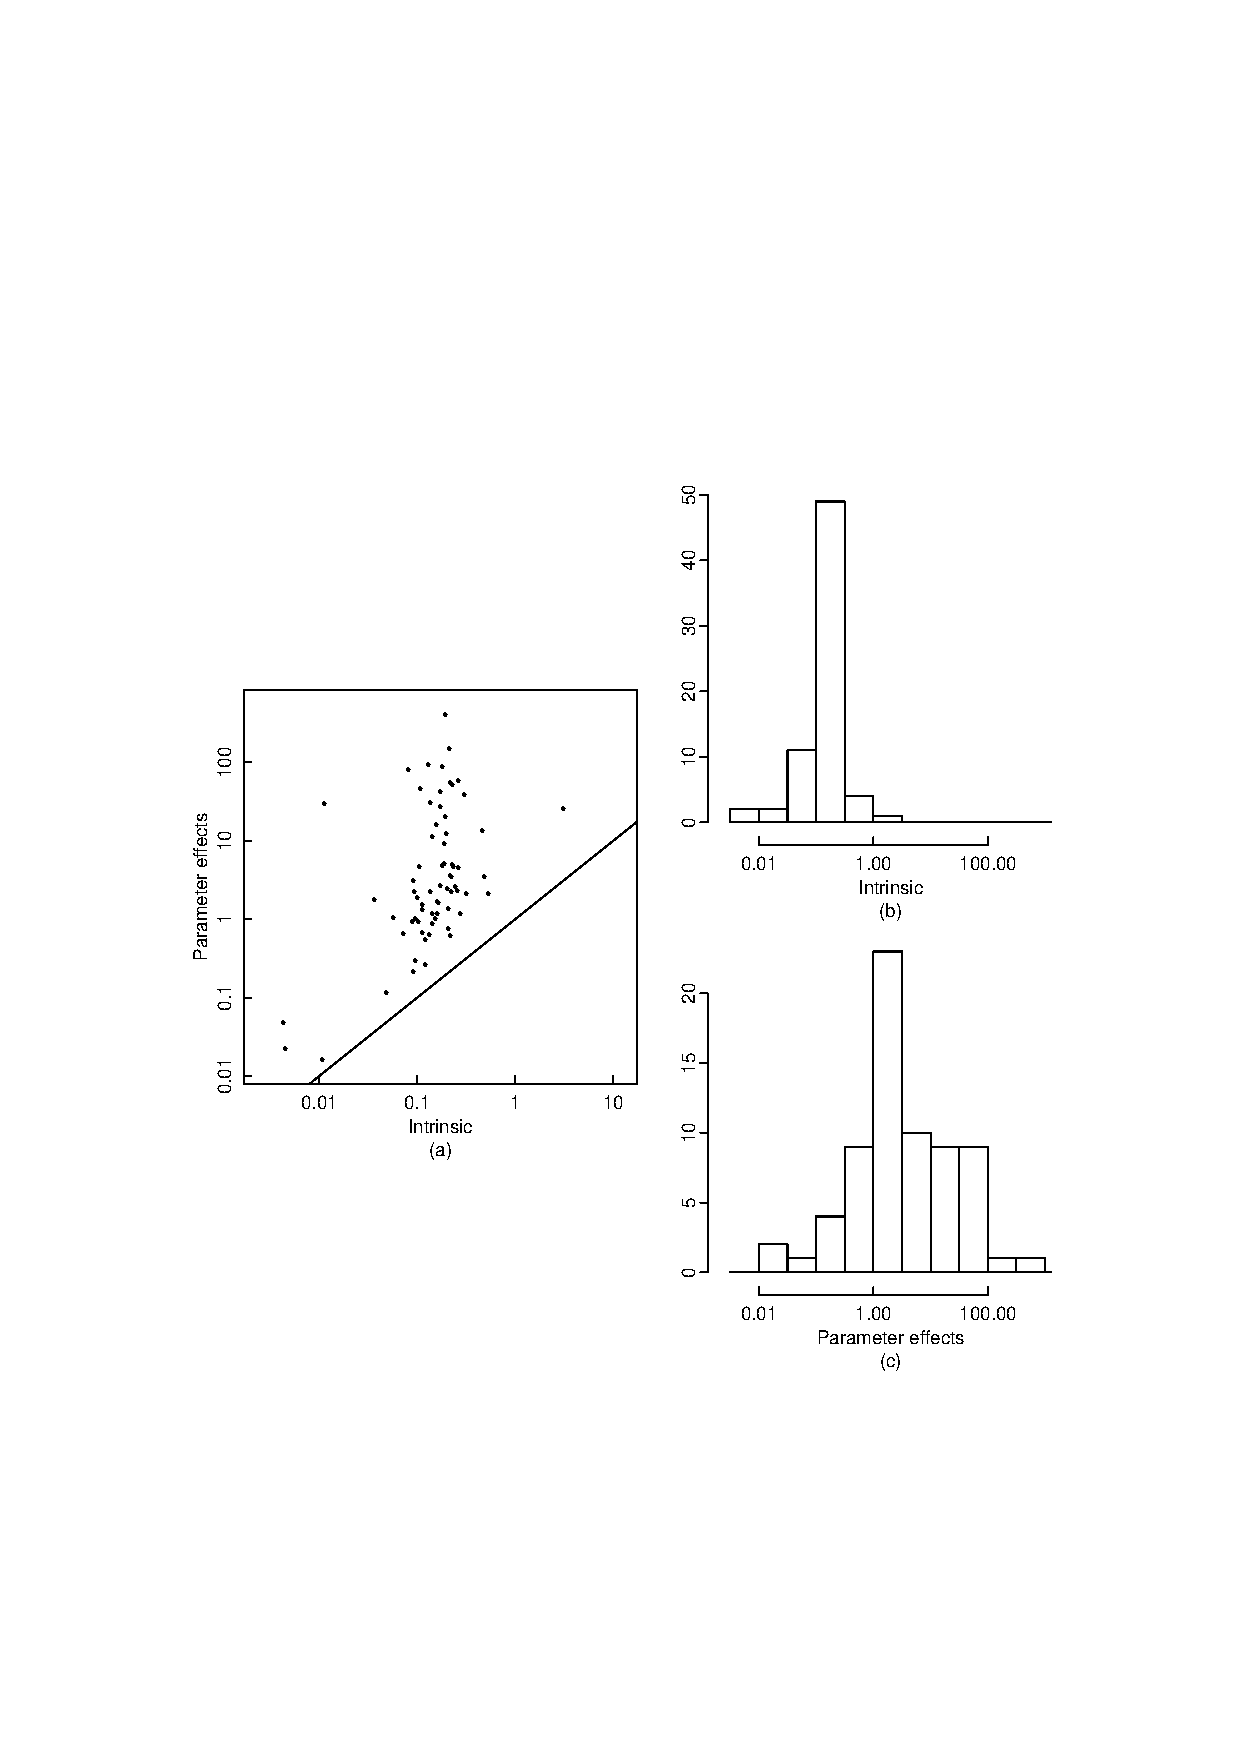
\includegraphics{7IntrinPE}%,width=\textwidth}
  \caption{\label{fig:IntrinPE}
  Histograms and scatterplots of scaled intrinsic and parameter
  effects curvatures for real data sets.  In part $a$, a scatterplot of
  the parameter effects versus intrinsic curvature is given.  The solid
  line is the line of equality.  Histograms of the curvatures are given
  in parts $b$ and $c$.}
\end{figure}
we present a scatterplot of the parameter
effects versus intrinsic $c \sqrt F$ values, and in
Figure \ref{fig:IntrinPE}$b$ and $c$
we show histograms of those values, all on log scales.
The solid line on Figure \ref{fig:IntrinPE}$a$ is the line of equality,
so that it is easily seen that the
intrinsic curvature is smaller, and in almost all cases very
much smaller, than the parameter effects curvature.
Figure \ref{fig:IntrinPE}$a$ also reveals that there is a positive
correlation between intrinsic and parameter effects nonlinearity.

Referring to the histograms,
it can be seen that the intrinsic curvature (Figure \ref{fig:IntrinPE}$b$)
is generally not large (about 93\% of the analyses have a
$c^{iota} \sqrt F $ value less than 0.3, which corresponds to
a 15\% deviation of the expectation surface from the
tangent plane).
Parameter effects curvatures, on the other hand, are often
bad (in only 10\% of the analyses is $c^{\theta} \sqrt F$ less than
0.3, which corresponds to a
deviation of less than 15\% from uniform coordinates,
and in about 80\% of the cases, the $c^{\theta} \sqrt F$ value is greater
than 1.0, which corresponds to a
deviation of a parameter curve from a straight line in excess of
100\%).

These results, based on real data sets from a variety of
sources, lead one to conclude that linear approximation
inference regions, which require the uniform coordinates assumption,
\index{assumptions!uniform coordinate}
\index{uniform coordinate!assumption}
can be very misleading in many practical situations.
They also lend strong support to the validity of the
planarity assumption which was used in deriving the
\index{planar assumption}
\index{assumptions!planar}
profile $t$ and profile pair plots in Chapter 6.
To further substantiate the validity of the planar
assumption, we investigate the effects of intrinsic nonlinearity
in more detail in the next section.

\section{Direct Assessment of the Effects of Intrinsic Nonlinearity}
\index{intrinsic nonlinearity!direct assessment}
\index{nonlinearity!intrinsic}

We have seen in the previous section that RMS
intrinsic curvatures are generally small, and so there is some
justification for assuming
that the planar assumption will be valid.
\index{planar assumption}
\index{assumptions!planar}
To give further justification, we look at the effects of
nonlinearity from a different viewpoint, by
considering that the construction of
a likelihood region involves two stages.
\index{likelihood!region}
In the first stage, we determine the intersection of the
expectation surface with the appropriate likelihood sphere
centered on $\by$, and in the second we map the coordinates of
that intersection into the parameter space.
A linear approximation confidence region is then obtained by
performing an approximation at each of these stages.
At the first stage, we replace the true expectation surface by a
plane, thereby producing a disk on the tangent plane, and at the
second stage we approximate the mapping of the disk to the
parameter plane by a linear mapping.
If the intrinsic nonlinearity is large, so that a tangent plane
does not provide an adequate approximation, we can use a
quadratic approximation \cite{hami:1980,hami:watt:bate:1982}.
%\glossary{ Hamilton, D.C.}
%\glossary{ Bates, D.M.}
%\glossary{ Watts, D.G.}

To obtain a quadratic approximation,
\index{expectation surface!quadratic approximation}
consider a point $\btheta$ in the parameter space.
This point maps through the nonlinear transformation,
$\boeta ( \btheta )$, to the point on the tangent plane with coordinates
$$
\btau = \bQ_1 \trans
[ \boeta ( \btheta )- \boeta ( \hat \btheta )]
$$
The coordinates $\btau$ provide a natural reference system for
the expectation surface,
in particular, a local set of coordinates with no
parameter effects nonlinearity.

An approximation to the expectation surface by a quadratic
surface centered at $ \boeta ( \hat \btheta )$ is
$$
\boeta ( \btau ) = \boeta ( \hat \btheta ) +
\bQ_1 \btau + { [ \bQ '_1 ][ \btau \trans \bC^{iota} \btau ]  
\over 2 }
$$
where $\bC$ is the relative curvature array and $\bQ_{1}$ and
$\bQ_{1}'$ are obtained from the $QR$ decomposition of the matrix
$\bD$ consisting of the first derivative and nonredundant second
derivative vectors (see Section 7.1).
Recall from Section 7.1.1 that the square brackets denote
matrix multiplication in which the summation is over the numerator
index.

An approximate expectation surface likelihood region and its
projection onto the tangent plane can then be defined by
rewriting equation (6.1) as
\begin{equation}
  { \bz \trans \bz \over \hat \bz \trans \hat \bz } = \left[ 1 +{P
  \over N -P}\FPNP\right]
  \label{eqn:8.13}
\end{equation}
and replacing the exact residual vector
$\bz ( \btheta ) = \by - \boeta$ with
the approximate residual vector
\index{residual!vector, approximate}
$\tilde \bz = \by - \tilde {\boeta}( \btau )$, where $\btau$ is a point on
the tangent plane in the coordinates given by the columns of $\bQ$.
Now the approximate residual vector at the point
$\tilde{\boeta}( \btau )$ is
$$
\tilde \bz = \hat \bz - \bQ_1 \btau -
{ [ \bQ '_1 ][ \btau \trans \bC^{iota} \btau ]   \over 2 }$$
and so
\begin{eqnarray}
  \bz \trans \bz&\approx&\tilde \bz \trans \tilde \bz\\
  \label{eqn:8.14}
  &=&\hat \bz \trans \hat \bz +
  \btau \trans ( \bI - \bB ) \btau +
  { ( \btau \trans \bC^{iota} \btau ) \trans
  ( \btau \trans \bC^{iota} \btau )   \over 4 }\nonumber
\end{eqnarray}
where $\bB=[ ( {\bQ'}_1\trans \hat \bz ) \trans ] [ \bC^{iota} ]$ is
the $P\times P$ matrix obtained from the inner product of the rotated
residual vector ${\bQ'}_1\trans \hat \bz$ and the intrinsic
curvature array.
The matrix $\bB$ is called the {\em effective residual curvature
matrix}, because it gives the effective
\index{matrix!effective residual curvature}
normal curvatures in the direction of the residual vector
$\hat \bz$ \cite{hami:watt:bate:1982}.
%\glossary{ Hamilton, D.C.}
%\glossary{ Watts, D.G.}
%\glossary{ Bates, D.M.}

Neglecting the term in (\ref{eqn:8.14}) which involves fourth powers of the
length of $\btau$ and inserting the first two terms into (\ref{eqn:8.13})
gives the approximate expectation surface region
\begin{equation}
  \btau \trans ( \bI-\bB ) \btau=\FPNP
  \label{eqn:8.15}
\end{equation}
Thus the tangent plane projection of the expectation surface
likelihood region is approximately an ellipsoid, since,
as shown below, $\bI - \bB$ is positive definite.
\citeasnoun{beal:1960} also noted that sum of
%\glossary{ Beale, E.M.L.}
squares contours were approximately ellipsoidal in the $\btau$
coordinates.
[\citeasnoun{hami:watt:bate:1982} obtained similar approximations
%\glossary{ Bates, D.M.}
%\glossary{ Hamilton, D.C.}
%\glossary{ Watts, D.G.}
to (\ref{eqn:8.15}) for confidence regions;
however, for reasons given in Chapter 6, we do not recommend
using confidence regions for nonlinear models.]

The tangent plane ellipsoids depend on the residual
vector--expectation surface configuration through the effective
residual curvature matrix $\bB$, whose entries give the projections
of the acceleration vectors on the residual vector.
If the expectation surface curves towards the residual vector, all
the projections are positive and all the eigenvalues of $\bB$ are
positive.
Consequently, the tangent plane ellipsoid is larger than the
linear approximation sphere.
This is intuitively correct because when the expectation surface
is curving towards the residual vector, more points on the
expectation surface are nearer the observation point than if the
expectation surface is a plane.
Similar reasoning holds when the expectation surface curves away
from the residual vector, causing the eigenvalues of $\bB$ to be
negative and the tangent plane ellipsoid to be smaller.

\begin{example}\label{bod:7}

Since the model for the BOD data is a 2-parameter model with a
conditionally linear parameter, the normal acceleration space has
dimension 1.
For these data,
$$
\bC^{iota} = \left[ \matrix {
\matrix{0 \cr 0}
\matrix{0 \cr 0.301}
}\right]
$$
and ${\bQ'}_1\trans\hat\bz=0.056$, so
$$
\bB = \left[ \matrix {
\matrix{0 \cr 0}
\matrix{0 \cr 0.017}
}\right]
$$
(Whenever the normal acceleration space is 1-dimensional, $\bB$
is a multiple of the single face in $\bC^{iota}$.)
The effective residual curvature is extremely small, indicating that the
expectation surface curves only slightly towards the observed response.
\end{example}

\citeasnoun{box:cout:1956} recommended using
%\glossary{ Box, G.E.P.}
%\glossary{ Coutie, G.A.}
$$
( \btheta - \hat \btheta ) \trans \bW ( \btheta - \hat \btheta )
$$
as an approximate confidence region for $\btheta$, where
$$
\bW = {1 \over 2 }\left. { \partial^2 S   \over  \partial
\btheta\partial \btheta \trans } \right|_{\hat {\theta}}
$$
In our notation,
\begin{eqnarray*}
  \bW&=&\dot \bV \trans \dot \bV -
  [ \hat \bz \trans ][ \ddot \bV ]\\
  &=&\bR_{11} \trans ( \bI - \bB ) \bR_{11}  
\end{eqnarray*}
so the inference region based on the second derivatives of the
sum of squares function may be considered the image, in parameter
space, of the ellipsoidal tangent plane likelihood region (\ref{eqn:8.15}),
assuming no parameter effects nonlinearity and with a linear
mapping from the tangent plane to the parameter plane.
Since $S( \hat \btheta )$ is a local minimum, it also follows that
$\bW$, and hence $\bI - \bB$, is positive definite.

A direct assessment of the effect of intrinsic nonlinearity on
likelihood regions can be made by calculating how much
the tangent plane inference ellipsoids differ from the
linear approximation spheres.
We do this by calculating the ratios of the lengths of the axes
of the ellipsoid to the radius of the linear approximation sphere.
The ratio for the $p $th axis is simply
$ \rho_p = ( 1 - \lambda_p )^{{-} {1\over 2}}$, where
$\lambda_p $ is the $p $th eigenvalue of $\bB$, and so
the {\em extreme axis length ratios}, $\rho_{1}$
and $\rho_{P}$, can be used as direct indicators of the
effects of intrinsic nonlinearity.
\index{intrinsic nonlinearity!direct assessment}

The last two columns of Table 7.2 give
the extreme axis length ratios for the 67 data set--model
combinations, and Figure~\ref{fig:Axisratio}
\begin{figure}
  \centerline{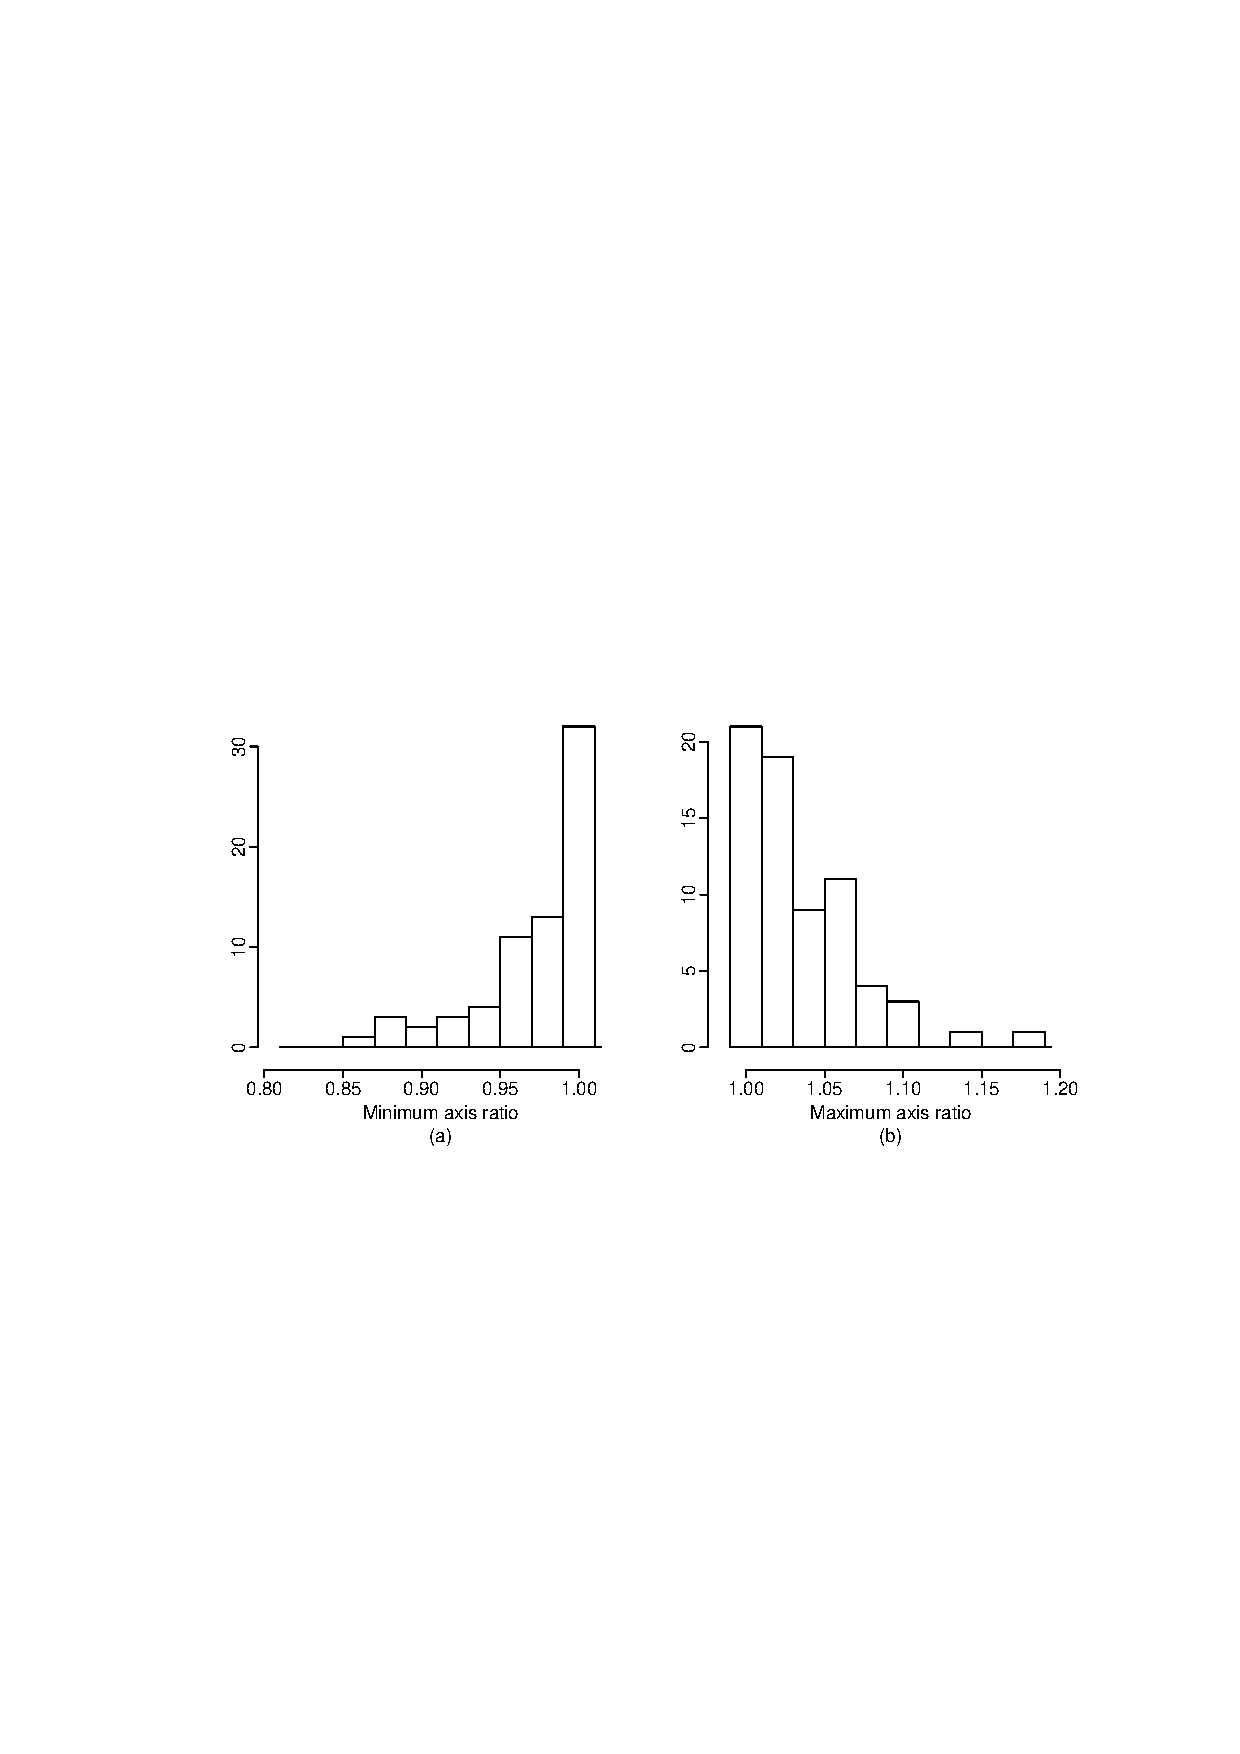
\includegraphics{7Axisratio}}%,height=2.25in}}
  \caption{\label{fig:Axisratio}
  Histograms of the minimum and maximum axis ratios for the 67 real
  data examples.  }
\end{figure}
presents histograms of these ratios.
From the data and the histograms
we see that the effect of intrinsic nonlinearity on
likelihood regions is extremely small,
with 95\% of the minimum axis ratios exceeding 0.9 and 80\%
exceeding 0.95.
Similarly, 97\% of the maximum axis
ratios are less than 1.1 and 70\% are less than 1.05.
The deviation of an ellipsoid from a sphere by 5 or 10\%
is quite small, and so we conclude that the planar assumption,
unlike the uniform coordinates assumption, will usually be
accurate and reliable.
For this reason we recommend summarizing the inferential results
of a nonlinear analysis by profile $t$ and profile pair plots,
since they only require the planar assumption.


% Local Variables: 
% mode: latex
% TeX-master: "nraia2"
% End: 
